\documentclass[]{article}
\usepackage{lmodern}
\usepackage{amssymb,amsmath}
\usepackage{ifxetex,ifluatex}
\usepackage{fixltx2e} % provides \textsubscript
\ifnum 0\ifxetex 1\fi\ifluatex 1\fi=0 % if pdftex
  \usepackage[T1]{fontenc}
  \usepackage[utf8]{inputenc}
\else % if luatex or xelatex
  \ifxetex
    \usepackage{mathspec}
  \else
    \usepackage{fontspec}
  \fi
  \defaultfontfeatures{Ligatures=TeX,Scale=MatchLowercase}
\fi
% use upquote if available, for straight quotes in verbatim environments
\IfFileExists{upquote.sty}{\usepackage{upquote}}{}
% use microtype if available
\IfFileExists{microtype.sty}{%
\usepackage{microtype}
\UseMicrotypeSet[protrusion]{basicmath} % disable protrusion for tt fonts
}{}
\usepackage[margin=1in]{geometry}
\usepackage{hyperref}
\hypersetup{unicode=true,
            pdfborder={0 0 0},
            breaklinks=true}
\urlstyle{same}  % don't use monospace font for urls
\usepackage{graphicx,grffile}
\makeatletter
\def\maxwidth{\ifdim\Gin@nat@width>\linewidth\linewidth\else\Gin@nat@width\fi}
\def\maxheight{\ifdim\Gin@nat@height>\textheight\textheight\else\Gin@nat@height\fi}
\makeatother
% Scale images if necessary, so that they will not overflow the page
% margins by default, and it is still possible to overwrite the defaults
% using explicit options in \includegraphics[width, height, ...]{}
\setkeys{Gin}{width=\maxwidth,height=\maxheight,keepaspectratio}
\IfFileExists{parskip.sty}{%
\usepackage{parskip}
}{% else
\setlength{\parindent}{0pt}
\setlength{\parskip}{6pt plus 2pt minus 1pt}
}
\setlength{\emergencystretch}{3em}  % prevent overfull lines
\providecommand{\tightlist}{%
  \setlength{\itemsep}{0pt}\setlength{\parskip}{0pt}}
\setcounter{secnumdepth}{0}
% Redefines (sub)paragraphs to behave more like sections
\ifx\paragraph\undefined\else
\let\oldparagraph\paragraph
\renewcommand{\paragraph}[1]{\oldparagraph{#1}\mbox{}}
\fi
\ifx\subparagraph\undefined\else
\let\oldsubparagraph\subparagraph
\renewcommand{\subparagraph}[1]{\oldsubparagraph{#1}\mbox{}}
\fi

%%% Use protect on footnotes to avoid problems with footnotes in titles
\let\rmarkdownfootnote\footnote%
\def\footnote{\protect\rmarkdownfootnote}

%%% Change title format to be more compact
\usepackage{titling}

% Create subtitle command for use in maketitle
\newcommand{\subtitle}[1]{
  \posttitle{
    \begin{center}\large#1\end{center}
    }
}

\setlength{\droptitle}{-2em}

  \title{}
    \pretitle{\vspace{\droptitle}}
  \posttitle{}
    \author{}
    \preauthor{}\postauthor{}
    \date{}
    \predate{}\postdate{}
  

\begin{document}

\newpage

\begin{figure}
\centering
\includegraphics[width=\textwidth]{Figure3.pdf}
\caption{Diagrammatic illustration of the ANTs longitudinal cortical thickness pipeline
for a single subject with $N$ time points.  From the $N$ original T1-weighted
images (left column, yellow panel) and the group template and priors (bottom row,
green panel), the single-subject template (SST) and auxiliary prior images
are created (center, blue panel).  These subject-specific template and other
auxiliary images are used to generate the individual time-point cortical
thickness maps, in the individual time point's native space (denoted as
``ANTs Native'' in the text).  Optionally, one can
rigidly transform the time-point images prior to segmentation and cortical thickness
estimation (right column, red panel).  This alternative processing scheme is referred
to as ``ANTs SST''.  For regional thickness values, regional labels
are propagated to each image using a given atlas set (with cortical labels)
and joint label fusion.}
\label{fig:pipeline}
\end{figure}

\newpage

\begin{figure}
\centering
\includegraphics[width=\textwidth]{Figure4.pdf}
\caption{Top row:  Canonical views of the template created from 52 randomly selected
cognitively normal subjects
of the ADNI-1 database.  The prior probability mask for the whole brain (middle row)
and the six tissue priors (bottom row) are used to ``seed'' each single-subject template for creation of
a probabilistic brain mask and probabilistic tissues priors during longitudinal
processing.}
\label{fig:template}
\end{figure}

\newpage

\begin{figure}[ht!]
\centering
\includegraphics[width=\textwidth]{Figure6.pdf}
\caption{95\% credible intervals of the region-specific variance ratios
$r^k=\tau_k/\sigma_k$ are presented for each processing method.  The ANTs
SST method dominates the others across the majority of
regions---its point estimates (posterior medians) are greater than those of the other
processing methods except for the left and right EC values in
FreeSurfer Long (although there is significant overlap in the credible intervals
in those regions).
These results also suggest that longitudinal processing is to be
preferred for both packages.}
\label{fig:ratios}
\end{figure}

\newpage

\begin{figure}[!h]
\centering
\includegraphics[width=\textwidth]{Figure7.pdf}
\caption{Box plots showing the distribution of the residual variability,
between subject variability, and ratio of the between-subject variability and
residual variability for each of the 62 DKT regions.  Note that the
``better'' measurement maximizes this latter ratio.}
\label{fig:variance_boxplots}
\end{figure}

\newpage

\begin{figure}[!h]
\centering
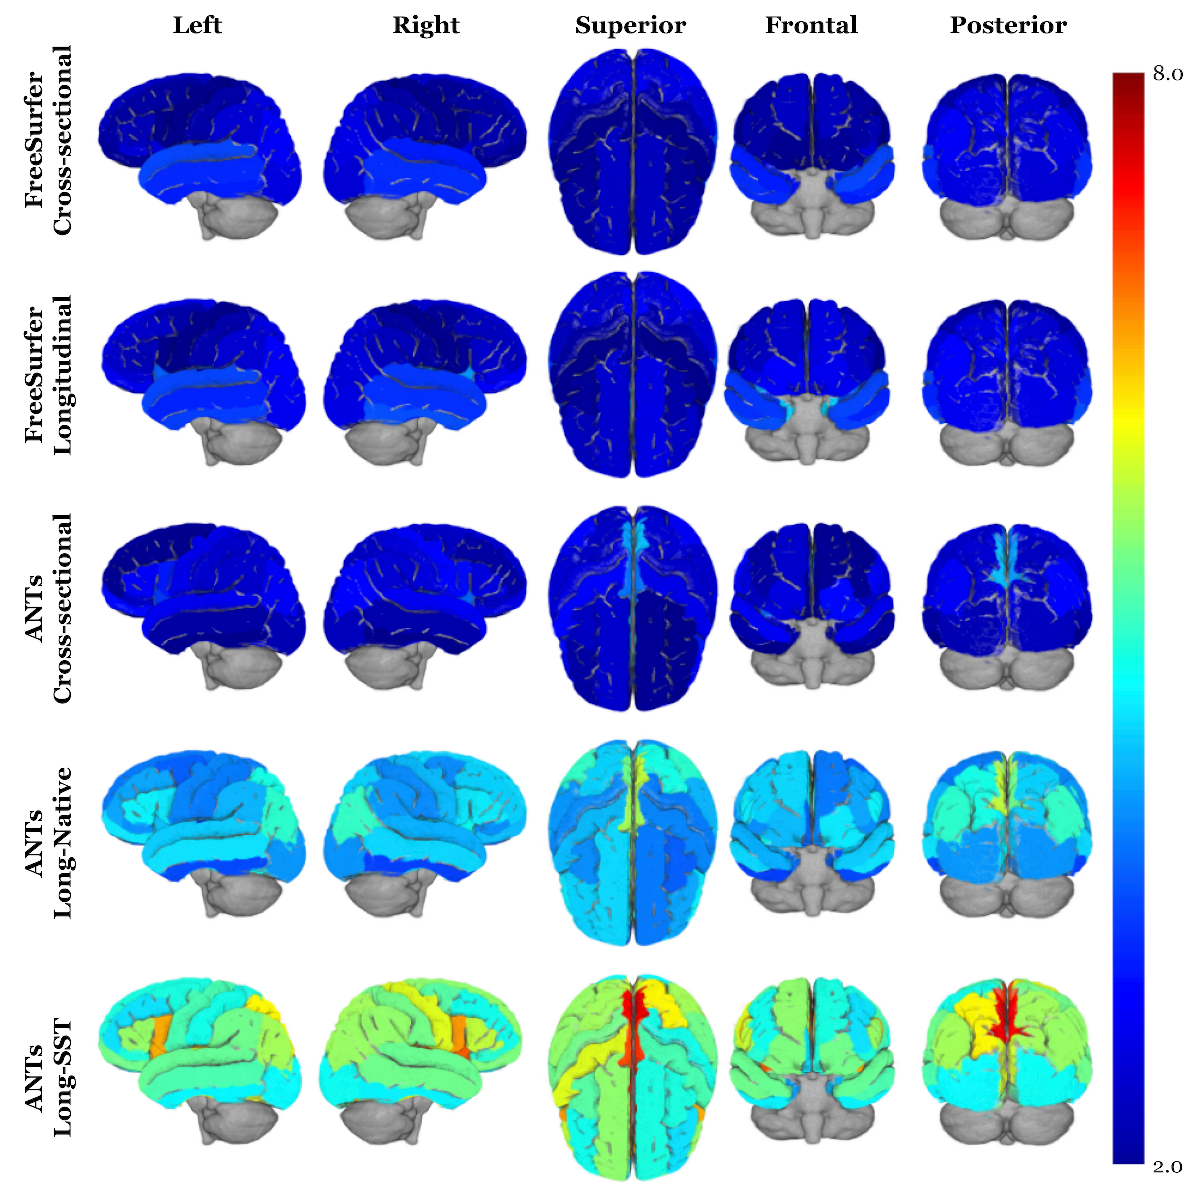
\includegraphics[width=\textwidth]{Figure8.pdf}
\caption{3-D volumetric rendering of the regional variance ratio values on the generated ADNI template.
The higher variance ratios indicate greater between-subject to residual variability.}
\label{fig:brain_variance}
\end{figure}

\newpage

\begin{figure}[ht!]
\centering
\includegraphics[width=1.0\textwidth]{Figure9.pdf}
\caption{
Log-scaled $p$-values summarizing Tables 2 and 3 demonstrating performance differences
across cross-sectional and longitudinal pipelines for the three diagnostic contrasts.
}
\label{fig:logpvalues}
\end{figure}

\newpage


\begin{table}[!htb]
\centering
\caption{The 31 cortical labels (per hemisphere) of the Desikan-Killiany-Tourville atlas.  }
\begin{tabular*}{0.75\textwidth}{@{\extracolsep{\fill}} l l}
  \toprule
  \midrule
  1) caudal anterior cingulate & 17) pars orbitalis \\
  2) caudal middle frontal & 18) pars triangularis \\
  3) cuneus &  19) pericalcarine \\
  4) entorhinal & 20) postcentral \\
  5) fusiform &  21) posterior cingulate\\
  6) inferior parietal & 22) precentral \\
  7) inferior temporal & 23) precuneus \\
  8) isthmus cingulate & 24) rosterior anterior cingulate\\
  9) lateral occipital & 25) rostral middle frontal \\
  10) lateral orbitofrontal  & 26) superior frontal \\
  11) lingual & 27) superior parietal \\
  12) medial orbitofrontal & 28) superior temporal \\
  13) middle temporal & 29) supramarginal \\
  14) parahippocampal & 30) transverse temporal \\
  15) paracentral & 31) insula \\
  16) pars opercularis  & {}\\
  \bottomrule
\end{tabular*}
\label{table:dkt_labels}
\end{table}


\newpage

\begin{table}

\caption{\label{tab:}95\% confidence intervals for the difference in slope values for the three diagnoses (CN, LMCI, AD) of the ADNI-1 data set for each DKT region of the left hemisphere.  Each cell is color-coded based on the adjusted log-scaled $p$-value significance from dark orange ($p$ < 1e-10) to yellow ($p$ = 0.1). Absence of color denotes nonsignificance.}
\centering
\resizebox{\linewidth}{!}{\begin{tabular}[t]{>{\bfseries}cccccccccccccccc}
\toprule
\multicolumn{1}{c}{\bfseries  } & \multicolumn{5}{c}{\bfseries LMCI$-$CN} & \multicolumn{5}{c}{\bfseries AD$-$LMCI} & \multicolumn{5}{c}{\bfseries AD$-$CN} \\
\cmidrule(l{2pt}r{2pt}){2-6} \cmidrule(l{2pt}r{2pt}){7-11} \cmidrule(l{2pt}r{2pt}){12-16}
\rotatebox{45}{DKT} & \rotatebox{45}{FSCross} & \rotatebox{45}{FSLong} & \rotatebox{45}{ANTsCross} & \rotatebox{45}{ANTsNative} & \rotatebox{45}{ANTsSST} & \rotatebox{45}{FSCross} & \rotatebox{45}{FSLong} & \rotatebox{45}{ANTsCross} & \rotatebox{45}{ANTsNative} & \rotatebox{45}{ANTsSST} & \rotatebox{45}{FSCross} & \rotatebox{45}{FSLong} & \rotatebox{45}{ANTsCross} & \rotatebox{45}{ANTsNative} & \rotatebox{45}{ANTsSST}\\
\midrule
lcACC  &  \cellcolor[HTML]{FFFFFF}{\textcolor{black}{-0.03,0.068}}  &  \cellcolor[HTML]{FFFFFF}{\textcolor{black}{-0.038,0.058}}  &  \cellcolor[HTML]{FFFFFF}{\textcolor{black}{-0.132,0.024}}  &  \cellcolor[HTML]{F4DF53}{\textcolor{black}{-0.235,-0.065}}  &  \cellcolor[HTML]{F4E054}{\textcolor{black}{-0.238,-0.065}}  &  \cellcolor[HTML]{FFFFFF}{\textcolor{black}{-0.075,0.033}}  &  \cellcolor[HTML]{FFFFFF}{\textcolor{black}{-0.08,0.024}}  &  \cellcolor[HTML]{FFFFFF}{\textcolor{black}{-0.103,0.068}}  &  \cellcolor[HTML]{F9FC9C}{\textcolor{black}{-0.187,-0.001}}  &  \cellcolor[HTML]{F3F78B}{\textcolor{black}{-0.211,-0.022}}  &  \cellcolor[HTML]{FFFFFF}{\textcolor{black}{-0.063,0.058}}  &  \cellcolor[HTML]{FFFFFF}{\textcolor{black}{-0.077,0.041}}  &  \cellcolor[HTML]{FFFFFF}{\textcolor{black}{-0.168,0.024}}  &  \cellcolor[HTML]{FBB519}{\textcolor{black}{-0.349,-0.14}}  &  \cellcolor[HTML]{FCA90E}{\textcolor{black}{-0.375,-0.162}}\\
lcMFG  &  \cellcolor[HTML]{FBBC21}{\textcolor{black}{-0.111,-0.043}}  &  \cellcolor[HTML]{FAC52B}{\textcolor{black}{-0.11,-0.04}}  &  \cellcolor[HTML]{F9CB35}{\textcolor{black}{-0.197,-0.067}}  &  \cellcolor[HTML]{F8CF3A}{\textcolor{black}{-0.188,-0.063}}  &  \cellcolor[HTML]{F7D23F}{\textcolor{black}{-0.188,-0.061}}  &  \cellcolor[HTML]{F6D745}{\textcolor{black}{-0.109,-0.034}}  &  \cellcolor[HTML]{FCB115}{\textcolor{black}{-0.13,-0.053}}  &  \cellcolor[HTML]{F4DC4E}{\textcolor{black}{-0.201,-0.058}}  &  \cellcolor[HTML]{F9CB35}{\textcolor{black}{-0.21,-0.073}}  &  \cellcolor[HTML]{F6D644}{\textcolor{black}{-0.201,-0.062}}  &  \cellcolor[HTML]{EA632A}{\textcolor{black}{-0.19,-0.106}}  &  \cellcolor[HTML]{EA632A}{\textcolor{black}{-0.21,-0.124}}  &  \cellcolor[HTML]{ED6825}{\textcolor{black}{-0.342,-0.182}}  &  \cellcolor[HTML]{EA632A}{\textcolor{black}{-0.345,-0.19}}  &  \cellcolor[HTML]{ED6825}{\textcolor{black}{-0.334,-0.178}}\\
lCUN  &  \cellcolor[HTML]{FFFFFF}{\textcolor{black}{-0.042,0.004}}  &  \cellcolor[HTML]{FBFEA3}{\textcolor{black}{-0.046,0.002}}  &  \cellcolor[HTML]{FFFFFF}{\textcolor{black}{-0.049,0.049}}  &  \cellcolor[HTML]{FFFFFF}{\textcolor{black}{-0.073,0.038}}  &  \cellcolor[HTML]{FFFFFF}{\textcolor{black}{-0.08,0.03}}  &  \cellcolor[HTML]{FFFFFF}{\textcolor{black}{-0.03,0.021}}  &  \cellcolor[HTML]{FFFFFF}{\textcolor{black}{-0.034,0.019}}  &  \cellcolor[HTML]{F9FC9D}{\textcolor{black}{-0.108,0}}  &  \cellcolor[HTML]{F3F689}{\textcolor{black}{-0.138,-0.016}}  &  \cellcolor[HTML]{F1F17A}{\textcolor{black}{-0.145,-0.024}}  &  \cellcolor[HTML]{FFFFFF}{\textcolor{black}{-0.053,0.005}}  &  \cellcolor[HTML]{F9FC9E}{\textcolor{black}{-0.059,0}}  &  \cellcolor[HTML]{FBFEA3}{\textcolor{black}{-0.115,0.006}}  &  \cellcolor[HTML]{F2F17B}{\textcolor{black}{-0.164,-0.026}}  &  \cellcolor[HTML]{F2E763}{\textcolor{black}{-0.177,-0.041}}\\
lENT  &  \cellcolor[HTML]{EA632A}{\textcolor{black}{-0.404,-0.24}}  &  \cellcolor[HTML]{EA632A}{\textcolor{black}{-0.405,-0.24}}  &  \cellcolor[HTML]{F1EE73}{\textcolor{black}{-0.285,-0.054}}  &  \cellcolor[HTML]{FB9706}{\textcolor{black}{-0.479,-0.219}}  &  \cellcolor[HTML]{FB9806}{\textcolor{black}{-0.486,-0.223}}  &  \cellcolor[HTML]{F67E14}{\textcolor{black}{-0.359,-0.179}}  &  \cellcolor[HTML]{F57B17}{\textcolor{black}{-0.385,-0.204}}  &  \cellcolor[HTML]{F4DE52}{\textcolor{black}{-0.354,-0.1}}  &  \cellcolor[HTML]{FBBD22}{\textcolor{black}{-0.462,-0.177}}  &  \cellcolor[HTML]{FCA50A}{\textcolor{black}{-0.514,-0.226}}  &  \cellcolor[HTML]{EA632A}{\textcolor{black}{-0.692,-0.489}}  &  \cellcolor[HTML]{EA632A}{\textcolor{black}{-0.719,-0.515}}  &  \cellcolor[HTML]{FA9207}{\textcolor{black}{-0.539,-0.254}}  &  \cellcolor[HTML]{EA632A}{\textcolor{black}{-0.83,-0.509}}  &  \cellcolor[HTML]{EA632A}{\textcolor{black}{-0.887,-0.562}}\\
lFUS  &  \cellcolor[HTML]{FB9B06}{\textcolor{black}{-0.129,-0.059}}  &  \cellcolor[HTML]{FCA60C}{\textcolor{black}{-0.126,-0.054}}  &  \cellcolor[HTML]{F2F482}{\textcolor{black}{-0.196,-0.029}}  &  \cellcolor[HTML]{FAC127}{\textcolor{black}{-0.308,-0.116}}  &  \cellcolor[HTML]{FBB71B}{\textcolor{black}{-0.321,-0.128}}  &  \cellcolor[HTML]{F8870E}{\textcolor{black}{-0.149,-0.073}}  &  \cellcolor[HTML]{F3761B}{\textcolor{black}{-0.161,-0.082}}  &  \cellcolor[HTML]{FAC127}{\textcolor{black}{-0.302,-0.117}}  &  \cellcolor[HTML]{FA9207}{\textcolor{black}{-0.398,-0.187}}  &  \cellcolor[HTML]{F68013}{\textcolor{black}{-0.418,-0.207}}  &  \cellcolor[HTML]{EA632A}{\textcolor{black}{-0.248,-0.162}}  &  \cellcolor[HTML]{EA632A}{\textcolor{black}{-0.255,-0.167}}  &  \cellcolor[HTML]{F2741C}{\textcolor{black}{-0.425,-0.218}}  &  \cellcolor[HTML]{EA632A}{\textcolor{black}{-0.623,-0.385}}  &  \cellcolor[HTML]{EA632A}{\textcolor{black}{-0.656,-0.418}}\\
lIPL  &  \cellcolor[HTML]{FAC42A}{\textcolor{black}{-0.099,-0.037}}  &  \cellcolor[HTML]{F9C931}{\textcolor{black}{-0.099,-0.035}}  &  \cellcolor[HTML]{F4DE50}{\textcolor{black}{-0.245,-0.069}}  &  \cellcolor[HTML]{F4DD4F}{\textcolor{black}{-0.245,-0.07}}  &  \cellcolor[HTML]{F4E054}{\textcolor{black}{-0.246,-0.067}}  &  \cellcolor[HTML]{F37818}{\textcolor{black}{-0.138,-0.07}}  &  \cellcolor[HTML]{F3771A}{\textcolor{black}{-0.144,-0.074}}  &  \cellcolor[HTML]{FB9A06}{\textcolor{black}{-0.357,-0.163}}  &  \cellcolor[HTML]{FB9C07}{\textcolor{black}{-0.349,-0.157}}  &  \cellcolor[HTML]{FCA90E}{\textcolor{black}{-0.344,-0.148}}  &  \cellcolor[HTML]{EA632A}{\textcolor{black}{-0.21,-0.134}}  &  \cellcolor[HTML]{EA632A}{\textcolor{black}{-0.215,-0.136}}  &  \cellcolor[HTML]{EA632A}{\textcolor{black}{-0.526,-0.308}}  &  \cellcolor[HTML]{EA632A}{\textcolor{black}{-0.52,-0.302}}  &  \cellcolor[HTML]{EA632A}{\textcolor{black}{-0.514,-0.292}}\\
lITG  &  \cellcolor[HTML]{F8890C}{\textcolor{black}{-0.146,-0.07}}  &  \cellcolor[HTML]{F98A0B}{\textcolor{black}{-0.148,-0.072}}  &  \cellcolor[HTML]{F6FA95}{\textcolor{black}{-0.225,-0.012}}  &  \cellcolor[HTML]{FAC52B}{\textcolor{black}{-0.359,-0.132}}  &  \cellcolor[HTML]{FCB317}{\textcolor{black}{-0.406,-0.165}}  &  \cellcolor[HTML]{F67E14}{\textcolor{black}{-0.165,-0.082}}  &  \cellcolor[HTML]{F8890C}{\textcolor{black}{-0.17,-0.086}}  &  \cellcolor[HTML]{FA9008}{\textcolor{black}{-0.454,-0.218}}  &  \cellcolor[HTML]{EC6726}{\textcolor{black}{-0.535,-0.286}}  &  \cellcolor[HTML]{EB6529}{\textcolor{black}{-0.574,-0.31}}  &  \cellcolor[HTML]{EA632A}{\textcolor{black}{-0.279,-0.185}}  &  \cellcolor[HTML]{EA632A}{\textcolor{black}{-0.285,-0.19}}  &  \cellcolor[HTML]{EB632A}{\textcolor{black}{-0.586,-0.322}}  &  \cellcolor[HTML]{EA632A}{\textcolor{black}{-0.797,-0.516}}  &  \cellcolor[HTML]{EA632A}{\textcolor{black}{-0.876,-0.579}}\\
liCC  &  \cellcolor[HTML]{F2EB6A}{\textcolor{black}{-0.091,-0.02}}  &  \cellcolor[HTML]{F1EB6C}{\textcolor{black}{-0.096,-0.02}}  &  \cellcolor[HTML]{F2F482}{\textcolor{black}{-0.17,-0.025}}  &  \cellcolor[HTML]{F8CD37}{\textcolor{black}{-0.252,-0.089}}  &  \cellcolor[HTML]{F9C933}{\textcolor{black}{-0.255,-0.089}}  &  \cellcolor[HTML]{F8D03B}{\textcolor{black}{-0.117,-0.039}}  &  \cellcolor[HTML]{FBBA1F}{\textcolor{black}{-0.137,-0.054}}  &  \cellcolor[HTML]{F6D746}{\textcolor{black}{-0.231,-0.071}}  &  \cellcolor[HTML]{FCAD11}{\textcolor{black}{-0.307,-0.129}}  &  \cellcolor[HTML]{FB9E07}{\textcolor{black}{-0.328,-0.147}}  &  \cellcolor[HTML]{F57A18}{\textcolor{black}{-0.177,-0.09}}  &  \cellcolor[HTML]{ED6925}{\textcolor{black}{-0.2,-0.107}}  &  \cellcolor[HTML]{FA9207}{\textcolor{black}{-0.338,-0.159}}  &  \cellcolor[HTML]{EA632A}{\textcolor{black}{-0.489,-0.288}}  &  \cellcolor[HTML]{EA632A}{\textcolor{black}{-0.512,-0.307}}\\
lLOG  &  \cellcolor[HTML]{F1EC6E}{\textcolor{black}{-0.065,-0.013}}  &  \cellcolor[HTML]{F2F27C}{\textcolor{black}{-0.062,-0.01}}  &  \cellcolor[HTML]{F4F78D}{\textcolor{black}{-0.172,-0.017}}  &  \cellcolor[HTML]{F2F27E}{\textcolor{black}{-0.18,-0.027}}  &  \cellcolor[HTML]{F3F587}{\textcolor{black}{-0.176,-0.021}}  &  \cellcolor[HTML]{F1EE73}{\textcolor{black}{-0.07,-0.013}}  &  \cellcolor[HTML]{F2E966}{\textcolor{black}{-0.074,-0.017}}  &  \cellcolor[HTML]{F9CB35}{\textcolor{black}{-0.262,-0.091}}  &  \cellcolor[HTML]{FCB014}{\textcolor{black}{-0.285,-0.119}}  &  \cellcolor[HTML]{FCA309}{\textcolor{black}{-0.304,-0.134}}  &  \cellcolor[HTML]{FCA70D}{\textcolor{black}{-0.112,-0.049}}  &  \cellcolor[HTML]{FCA70D}{\textcolor{black}{-0.113,-0.049}}  &  \cellcolor[HTML]{F98C0A}{\textcolor{black}{-0.367,-0.175}}  &  \cellcolor[HTML]{EE6A24}{\textcolor{black}{-0.399,-0.211}}  &  \cellcolor[HTML]{EB6628}{\textcolor{black}{-0.413,-0.222}}\\
lLOF  &  \cellcolor[HTML]{F9FC9C}{\textcolor{black}{-0.062,0}}  &  \cellcolor[HTML]{F2F27E}{\textcolor{black}{-0.071,-0.011}}  &  \cellcolor[HTML]{F9FC9D}{\textcolor{black}{-0.153,0}}  &  \cellcolor[HTML]{F5DB4C}{\textcolor{black}{-0.23,-0.068}}  &  \cellcolor[HTML]{F5DB4C}{\textcolor{black}{-0.236,-0.069}}  &  \cellcolor[HTML]{F3F586}{\textcolor{black}{-0.078,-0.01}}  &  \cellcolor[HTML]{F2E763}{\textcolor{black}{-0.086,-0.02}}  &  \cellcolor[HTML]{F2EA69}{\textcolor{black}{-0.217,-0.048}}  &  \cellcolor[HTML]{FAC62E}{\textcolor{black}{-0.279,-0.101}}  &  \cellcolor[HTML]{FCB317}{\textcolor{black}{-0.31,-0.127}}  &  \cellcolor[HTML]{F7D340}{\textcolor{black}{-0.114,-0.037}}  &  \cellcolor[HTML]{FCA50A}{\textcolor{black}{-0.131,-0.057}}  &  \cellcolor[HTML]{FAC026}{\textcolor{black}{-0.303,-0.114}}  &  \cellcolor[HTML]{EB6429}{\textcolor{black}{-0.439,-0.239}}  &  \cellcolor[HTML]{EA632A}{\textcolor{black}{-0.474,-0.269}}\\
lLING  &  \cellcolor[HTML]{FFFFFF}{\textcolor{black}{-0.041,0.005}}  &  \cellcolor[HTML]{FFFFFF}{\textcolor{black}{-0.041,0.004}}  &  \cellcolor[HTML]{FFFFFF}{\textcolor{black}{-0.097,0.033}}  &  \cellcolor[HTML]{F8FB9B}{\textcolor{black}{-0.148,-0.003}}  &  \cellcolor[HTML]{F4F78D}{\textcolor{black}{-0.157,-0.015}}  &  \cellcolor[HTML]{F2E967}{\textcolor{black}{-0.065,-0.015}}  &  \cellcolor[HTML]{F4DE52}{\textcolor{black}{-0.07,-0.02}}  &  \cellcolor[HTML]{FAFD9F}{\textcolor{black}{-0.141,0.003}}  &  \cellcolor[HTML]{F3F584}{\textcolor{black}{-0.184,-0.024}}  &  \cellcolor[HTML]{F1EF75}{\textcolor{black}{-0.19,-0.035}}  &  \cellcolor[HTML]{F9CB35}{\textcolor{black}{-0.086,-0.03}}  &  \cellcolor[HTML]{FBBD22}{\textcolor{black}{-0.091,-0.035}}  &  \cellcolor[HTML]{F3F689}{\textcolor{black}{-0.181,-0.02}}  &  \cellcolor[HTML]{F8CF3A}{\textcolor{black}{-0.269,-0.09}}  &  \cellcolor[HTML]{FBBE23}{\textcolor{black}{-0.285,-0.111}}\\
lMOF  &  \cellcolor[HTML]{F2F482}{\textcolor{black}{-0.079,-0.011}}  &  \cellcolor[HTML]{F6D542}{\textcolor{black}{-0.095,-0.03}}  &  \cellcolor[HTML]{F8FB9B}{\textcolor{black}{-0.181,-0.004}}  &  \cellcolor[HTML]{FBBC21}{\textcolor{black}{-0.294,-0.114}}  &  \cellcolor[HTML]{FAC329}{\textcolor{black}{-0.303,-0.114}}  &  \cellcolor[HTML]{F5F994}{\textcolor{black}{-0.08,-0.005}}  &  \cellcolor[HTML]{F1F178}{\textcolor{black}{-0.086,-0.015}}  &  \cellcolor[HTML]{F2E865}{\textcolor{black}{-0.255,-0.059}}  &  \cellcolor[HTML]{FBBD22}{\textcolor{black}{-0.326,-0.128}}  &  \cellcolor[HTML]{FB9B06}{\textcolor{black}{-0.378,-0.171}}  &  \cellcolor[HTML]{F9CB35}{\textcolor{black}{-0.13,-0.046}}  &  \cellcolor[HTML]{F98C0A}{\textcolor{black}{-0.153,-0.073}}  &  \cellcolor[HTML]{FBBC21}{\textcolor{black}{-0.359,-0.139}}  &  \cellcolor[HTML]{EA632A}{\textcolor{black}{-0.542,-0.32}}  &  \cellcolor[HTML]{EA632A}{\textcolor{black}{-0.599,-0.367}}\\
lMGH  &  \cellcolor[HTML]{F2741C}{\textcolor{black}{-0.147,-0.076}}  &  \cellcolor[HTML]{F98B0B}{\textcolor{black}{-0.137,-0.066}}  &  \cellcolor[HTML]{F3E55E}{\textcolor{black}{-0.239,-0.06}}  &  \cellcolor[HTML]{FC9F07}{\textcolor{black}{-0.32,-0.142}}  &  \cellcolor[HTML]{FB9606}{\textcolor{black}{-0.35,-0.161}}  &  \cellcolor[HTML]{EE6A24}{\textcolor{black}{-0.166,-0.088}}  &  \cellcolor[HTML]{EC6726}{\textcolor{black}{-0.167,-0.089}}  &  \cellcolor[HTML]{FCA007}{\textcolor{black}{-0.361,-0.162}}  &  \cellcolor[HTML]{EA632A}{\textcolor{black}{-0.442,-0.247}}  &  \cellcolor[HTML]{EA632A}{\textcolor{black}{-0.471,-0.265}}  &  \cellcolor[HTML]{EA632A}{\textcolor{black}{-0.283,-0.194}}  &  \cellcolor[HTML]{EA632A}{\textcolor{black}{-0.274,-0.186}}  &  \cellcolor[HTML]{EA632A}{\textcolor{black}{-0.523,-0.3}}  &  \cellcolor[HTML]{EA632A}{\textcolor{black}{-0.686,-0.465}}  &  \cellcolor[HTML]{EA632A}{\textcolor{black}{-0.74,-0.506}}\\
lPARH  &  \cellcolor[HTML]{F5DB4C}{\textcolor{black}{-0.151,-0.044}}  &  \cellcolor[HTML]{F3E35A}{\textcolor{black}{-0.137,-0.036}}  &  \cellcolor[HTML]{F3F689}{\textcolor{black}{-0.189,-0.022}}  &  \cellcolor[HTML]{F4DD4F}{\textcolor{black}{-0.26,-0.074}}  &  \cellcolor[HTML]{F5DC4D}{\textcolor{black}{-0.265,-0.077}}  &  \cellcolor[HTML]{FAC127}{\textcolor{black}{-0.189,-0.071}}  &  \cellcolor[HTML]{FABF25}{\textcolor{black}{-0.182,-0.07}}  &  \cellcolor[HTML]{FBBD22}{\textcolor{black}{-0.301,-0.116}}  &  \cellcolor[HTML]{FCAA0F}{\textcolor{black}{-0.355,-0.152}}  &  \cellcolor[HTML]{FCA007}{\textcolor{black}{-0.37,-0.164}}  &  \cellcolor[HTML]{EB632A}{\textcolor{black}{-0.294,-0.161}}  &  \cellcolor[HTML]{EB6429}{\textcolor{black}{-0.275,-0.15}}  &  \cellcolor[HTML]{F47918}{\textcolor{black}{-0.417,-0.211}}  &  \cellcolor[HTML]{EA632A}{\textcolor{black}{-0.536,-0.306}}  &  \cellcolor[HTML]{EA632A}{\textcolor{black}{-0.554,-0.322}}\\
lparaC  &  \cellcolor[HTML]{F2F482}{\textcolor{black}{-0.075,-0.011}}  &  \cellcolor[HTML]{F2E662}{\textcolor{black}{-0.088,-0.021}}  &  \cellcolor[HTML]{FFFFFF}{\textcolor{black}{-0.075,0.024}}  &  \cellcolor[HTML]{FFFFFF}{\textcolor{black}{-0.087,0.027}}  &  \cellcolor[HTML]{FFFFFF}{\textcolor{black}{-0.087,0.027}}  &  \cellcolor[HTML]{FFFFFF}{\textcolor{black}{-0.037,0.034}}  &  \cellcolor[HTML]{FFFFFF}{\textcolor{black}{-0.068,0.006}}  &  \cellcolor[HTML]{F8FB9B}{\textcolor{black}{-0.111,-0.002}}  &  \cellcolor[HTML]{FFFFFF}{\textcolor{black}{-0.114,0.011}}  &  \cellcolor[HTML]{FAFDA1}{\textcolor{black}{-0.122,0.003}}  &  \cellcolor[HTML]{F6FA95}{\textcolor{black}{-0.084,-0.005}}  &  \cellcolor[HTML]{F9CB35}{\textcolor{black}{-0.127,-0.044}}  &  \cellcolor[HTML]{F2F380}{\textcolor{black}{-0.143,-0.021}}  &  \cellcolor[HTML]{F5F991}{\textcolor{black}{-0.152,-0.011}}  &  \cellcolor[HTML]{F3F587}{\textcolor{black}{-0.16,-0.019}}\\
lpOPER  &  \cellcolor[HTML]{F4F78D}{\textcolor{black}{-0.07,-0.007}}  &  \cellcolor[HTML]{F2F482}{\textcolor{black}{-0.074,-0.011}}  &  \cellcolor[HTML]{F8CD37}{\textcolor{black}{-0.188,-0.065}}  &  \cellcolor[HTML]{FCA007}{\textcolor{black}{-0.222,-0.099}}  &  \cellcolor[HTML]{FCA70D}{\textcolor{black}{-0.211,-0.091}}  &  \cellcolor[HTML]{F8FB99}{\textcolor{black}{-0.072,-0.002}}  &  \cellcolor[HTML]{F3F587}{\textcolor{black}{-0.08,-0.01}}  &  \cellcolor[HTML]{F9C931}{\textcolor{black}{-0.212,-0.076}}  &  \cellcolor[HTML]{FBBE23}{\textcolor{black}{-0.218,-0.084}}  &  \cellcolor[HTML]{FAC026}{\textcolor{black}{-0.212,-0.08}}  &  \cellcolor[HTML]{F6D542}{\textcolor{black}{-0.115,-0.037}}  &  \cellcolor[HTML]{FABF25}{\textcolor{black}{-0.127,-0.048}}  &  \cellcolor[HTML]{EA632A}{\textcolor{black}{-0.346,-0.194}}  &  \cellcolor[HTML]{EA632A}{\textcolor{black}{-0.387,-0.236}}  &  \cellcolor[HTML]{EA632A}{\textcolor{black}{-0.371,-0.223}}\\
lpORB  &  \cellcolor[HTML]{F5DB4C}{\textcolor{black}{-0.105,-0.031}}  &  \cellcolor[HTML]{F4E258}{\textcolor{black}{-0.099,-0.026}}  &  \cellcolor[HTML]{FBFEA3}{\textcolor{black}{-0.163,0.007}}  &  \cellcolor[HTML]{F1ED70}{\textcolor{black}{-0.203,-0.041}}  &  \cellcolor[HTML]{F1EC6E}{\textcolor{black}{-0.205,-0.042}}  &  \cellcolor[HTML]{FFFFFF}{\textcolor{black}{-0.053,0.028}}  &  \cellcolor[HTML]{FFFFFF}{\textcolor{black}{-0.067,0.014}}  &  \cellcolor[HTML]{F2F17B}{\textcolor{black}{-0.225,-0.037}}  &  \cellcolor[HTML]{F4E156}{\textcolor{black}{-0.244,-0.066}}  &  \cellcolor[HTML]{F8D03B}{\textcolor{black}{-0.267,-0.088}}  &  \cellcolor[HTML]{F4E054}{\textcolor{black}{-0.126,-0.034}}  &  \cellcolor[HTML]{F7D13D}{\textcolor{black}{-0.134,-0.044}}  &  \cellcolor[HTML]{F7D13D}{\textcolor{black}{-0.314,-0.104}}  &  \cellcolor[HTML]{FA9407}{\textcolor{black}{-0.377,-0.176}}  &  \cellcolor[HTML]{F57D15}{\textcolor{black}{-0.402,-0.2}}\\
lpTRI  &  \cellcolor[HTML]{FAC62D}{\textcolor{black}{-0.094,-0.035}}  &  \cellcolor[HTML]{FBBD22}{\textcolor{black}{-0.099,-0.038}}  &  \cellcolor[HTML]{F2F27C}{\textcolor{black}{-0.183,-0.029}}  &  \cellcolor[HTML]{F6D542}{\textcolor{black}{-0.209,-0.066}}  &  \cellcolor[HTML]{F2E662}{\textcolor{black}{-0.191,-0.046}}  &  \cellcolor[HTML]{F3F78B}{\textcolor{black}{-0.073,-0.008}}  &  \cellcolor[HTML]{F1ED71}{\textcolor{black}{-0.083,-0.016}}  &  \cellcolor[HTML]{F2EB6A}{\textcolor{black}{-0.217,-0.047}}  &  \cellcolor[HTML]{F6D543}{\textcolor{black}{-0.229,-0.072}}  &  \cellcolor[HTML]{F8CF3A}{\textcolor{black}{-0.24,-0.081}}  &  \cellcolor[HTML]{F8890C}{\textcolor{black}{-0.142,-0.068}}  &  \cellcolor[HTML]{F17020}{\textcolor{black}{-0.155,-0.08}}  &  \cellcolor[HTML]{FCA70D}{\textcolor{black}{-0.333,-0.143}}  &  \cellcolor[HTML]{ED6925}{\textcolor{black}{-0.377,-0.2}}  &  \cellcolor[HTML]{F3761B}{\textcolor{black}{-0.369,-0.189}}\\
lperiCAL  &  \cellcolor[HTML]{FFFFFF}{\textcolor{black}{-0.019,0.021}}  &  \cellcolor[HTML]{FFFFFF}{\textcolor{black}{-0.031,0.016}}  &  \cellcolor[HTML]{FFFFFF}{\textcolor{black}{-0.06,0.065}}  &  \cellcolor[HTML]{FFFFFF}{\textcolor{black}{-0.079,0.058}}  &  \cellcolor[HTML]{FFFFFF}{\textcolor{black}{-0.095,0.042}}  &  \cellcolor[HTML]{FFFFFF}{\textcolor{black}{-0.028,0.017}}  &  \cellcolor[HTML]{FFFFFF}{\textcolor{black}{-0.044,0.008}}  &  \cellcolor[HTML]{F1F077}{\textcolor{black}{-0.168,-0.03}}  &  \cellcolor[HTML]{F1EC6D}{\textcolor{black}{-0.19,-0.04}}  &  \cellcolor[HTML]{F4DF53}{\textcolor{black}{-0.207,-0.057}}  &  \cellcolor[HTML]{FFFFFF}{\textcolor{black}{-0.029,0.021}}  &  \cellcolor[HTML]{FBFEA3}{\textcolor{black}{-0.055,0.003}}  &  \cellcolor[HTML]{F3F68A}{\textcolor{black}{-0.174,-0.019}}  &  \cellcolor[HTML]{F1EE73}{\textcolor{black}{-0.211,-0.041}}  &  \cellcolor[HTML]{F6D746}{\textcolor{black}{-0.243,-0.074}}\\
lpostC  &  \cellcolor[HTML]{F8FB9B}{\textcolor{black}{-0.05,-0.001}}  &  \cellcolor[HTML]{F9FC9C}{\textcolor{black}{-0.052,-0.001}}  &  \cellcolor[HTML]{F3E55E}{\textcolor{black}{-0.12,-0.03}}  &  \cellcolor[HTML]{F3F689}{\textcolor{black}{-0.109,-0.012}}  &  \cellcolor[HTML]{F5F991}{\textcolor{black}{-0.11,-0.009}}  &  \cellcolor[HTML]{FFFFFF}{\textcolor{black}{-0.051,0.004}}  &  \cellcolor[HTML]{F4F88E}{\textcolor{black}{-0.062,-0.005}}  &  \cellcolor[HTML]{F2E763}{\textcolor{black}{-0.13,-0.03}}  &  \cellcolor[HTML]{F2E763}{\textcolor{black}{-0.14,-0.033}}  &  \cellcolor[HTML]{F2EA69}{\textcolor{black}{-0.143,-0.031}}  &  \cellcolor[HTML]{F2E763}{\textcolor{black}{-0.08,-0.019}}  &  \cellcolor[HTML]{F6D746}{\textcolor{black}{-0.092,-0.028}}  &  \cellcolor[HTML]{F98E09}{\textcolor{black}{-0.211,-0.1}}  &  \cellcolor[HTML]{FBB61A}{\textcolor{black}{-0.207,-0.087}}  &  \cellcolor[HTML]{FBB71B}{\textcolor{black}{-0.209,-0.084}}\\
lPCC  &  \cellcolor[HTML]{FFFFFF}{\textcolor{black}{-0.058,0.004}}  &  \cellcolor[HTML]{F6FA97}{\textcolor{black}{-0.068,-0.003}}  &  \cellcolor[HTML]{F1F17A}{\textcolor{black}{-0.157,-0.026}}  &  \cellcolor[HTML]{FBB71C}{\textcolor{black}{-0.258,-0.103}}  &  \cellcolor[HTML]{FABF25}{\textcolor{black}{-0.267,-0.104}}  &  \cellcolor[HTML]{F4F990}{\textcolor{black}{-0.075,-0.006}}  &  \cellcolor[HTML]{F2F27E}{\textcolor{black}{-0.084,-0.013}}  &  \cellcolor[HTML]{F1EE74}{\textcolor{black}{-0.177,-0.033}}  &  \cellcolor[HTML]{F6D847}{\textcolor{black}{-0.244,-0.074}}  &  \cellcolor[HTML]{F9CB35}{\textcolor{black}{-0.272,-0.093}}  &  \cellcolor[HTML]{F4E054}{\textcolor{black}{-0.106,-0.029}}  &  \cellcolor[HTML]{F9C830}{\textcolor{black}{-0.124,-0.044}}  &  \cellcolor[HTML]{FCAE12}{\textcolor{black}{-0.278,-0.116}}  &  \cellcolor[HTML]{EA632A}{\textcolor{black}{-0.436,-0.244}}  &  \cellcolor[HTML]{EA632A}{\textcolor{black}{-0.469,-0.267}}\\
lPreC  &  \cellcolor[HTML]{F3E55C}{\textcolor{black}{-0.092,-0.023}}  &  \cellcolor[HTML]{F5DB4C}{\textcolor{black}{-0.101,-0.03}}  &  \cellcolor[HTML]{FAC026}{\textcolor{black}{-0.145,-0.055}}  &  \cellcolor[HTML]{F3E35A}{\textcolor{black}{-0.138,-0.036}}  &  \cellcolor[HTML]{F1ED70}{\textcolor{black}{-0.135,-0.027}}  &  \cellcolor[HTML]{F9FC9C}{\textcolor{black}{-0.077,-0.001}}  &  \cellcolor[HTML]{F2F482}{\textcolor{black}{-0.093,-0.013}}  &  \cellcolor[HTML]{F5DB4C}{\textcolor{black}{-0.141,-0.042}}  &  \cellcolor[HTML]{F2EA69}{\textcolor{black}{-0.145,-0.032}}  &  \cellcolor[HTML]{F2F27E}{\textcolor{black}{-0.139,-0.021}}  &  \cellcolor[HTML]{FBBC21}{\textcolor{black}{-0.139,-0.054}}  &  \cellcolor[HTML]{FB9906}{\textcolor{black}{-0.162,-0.074}}  &  \cellcolor[HTML]{EB632A}{\textcolor{black}{-0.247,-0.136}}  &  \cellcolor[HTML]{FA9207}{\textcolor{black}{-0.239,-0.112}}  &  \cellcolor[HTML]{FCB317}{\textcolor{black}{-0.228,-0.095}}\\
lPCUN  &  \cellcolor[HTML]{FCA90E}{\textcolor{black}{-0.099,-0.042}}  &  \cellcolor[HTML]{FCB115}{\textcolor{black}{-0.105,-0.045}}  &  \cellcolor[HTML]{F2E660}{\textcolor{black}{-0.17,-0.041}}  &  \cellcolor[HTML]{F3E55C}{\textcolor{black}{-0.199,-0.05}}  &  \cellcolor[HTML]{F2E966}{\textcolor{black}{-0.197,-0.045}}  &  \cellcolor[HTML]{F6D542}{\textcolor{black}{-0.091,-0.028}}  &  \cellcolor[HTML]{FCB519}{\textcolor{black}{-0.112,-0.046}}  &  \cellcolor[HTML]{F7D23F}{\textcolor{black}{-0.208,-0.067}}  &  \cellcolor[HTML]{F7D340}{\textcolor{black}{-0.241,-0.078}}  &  \cellcolor[HTML]{F7D23E}{\textcolor{black}{-0.245,-0.08}}  &  \cellcolor[HTML]{EA632A}{\textcolor{black}{-0.165,-0.095}}  &  \cellcolor[HTML]{EA632A}{\textcolor{black}{-0.191,-0.117}}  &  \cellcolor[HTML]{F3771A}{\textcolor{black}{-0.323,-0.164}}  &  \cellcolor[HTML]{F2741C}{\textcolor{black}{-0.376,-0.193}}  &  \cellcolor[HTML]{F57B17}{\textcolor{black}{-0.378,-0.19}}\\
lrACC  &  \cellcolor[HTML]{F9FC9E}{\textcolor{black}{-0.088,0.001}}  &  \cellcolor[HTML]{F3F68A}{\textcolor{black}{-0.095,-0.011}}  &  \cellcolor[HTML]{FFFFFF}{\textcolor{black}{-0.133,0.05}}  &  \cellcolor[HTML]{F1ED71}{\textcolor{black}{-0.253,-0.05}}  &  \cellcolor[HTML]{F1F17A}{\textcolor{black}{-0.249,-0.042}}  &  \cellcolor[HTML]{FFFFFF}{\textcolor{black}{-0.054,0.044}}  &  \cellcolor[HTML]{FFFFFF}{\textcolor{black}{-0.054,0.039}}  &  \cellcolor[HTML]{FFFFFF}{\textcolor{black}{-0.151,0.05}}  &  \cellcolor[HTML]{F2F17B}{\textcolor{black}{-0.266,-0.044}}  &  \cellcolor[HTML]{F4E156}{\textcolor{black}{-0.308,-0.083}}  &  \cellcolor[HTML]{FFFFFF}{\textcolor{black}{-0.103,0.007}}  &  \cellcolor[HTML]{F5F991}{\textcolor{black}{-0.113,-0.008}}  &  \cellcolor[HTML]{FFFFFF}{\textcolor{black}{-0.205,0.021}}  &  \cellcolor[HTML]{FCAB11}{\textcolor{black}{-0.431,-0.182}}  &  \cellcolor[HTML]{FB9706}{\textcolor{black}{-0.468,-0.214}}\\
lrMFG  &  \cellcolor[HTML]{FAC228}{\textcolor{black}{-0.087,-0.032}}  &  \cellcolor[HTML]{FCAE12}{\textcolor{black}{-0.095,-0.039}}  &  \cellcolor[HTML]{F2EA69}{\textcolor{black}{-0.247,-0.054}}  &  \cellcolor[HTML]{FBBE23}{\textcolor{black}{-0.293,-0.115}}  &  \cellcolor[HTML]{FAC62D}{\textcolor{black}{-0.297,-0.108}}  &  \cellcolor[HTML]{F6D745}{\textcolor{black}{-0.087,-0.027}}  &  \cellcolor[HTML]{F6D847}{\textcolor{black}{-0.089,-0.027}}  &  \cellcolor[HTML]{F4E156}{\textcolor{black}{-0.292,-0.078}}  &  \cellcolor[HTML]{F9C931}{\textcolor{black}{-0.302,-0.106}}  &  \cellcolor[HTML]{FAC127}{\textcolor{black}{-0.332,-0.125}}  &  \cellcolor[HTML]{EA632A}{\textcolor{black}{-0.151,-0.083}}  &  \cellcolor[HTML]{EA632A}{\textcolor{black}{-0.16,-0.091}}  &  \cellcolor[HTML]{F98E09}{\textcolor{black}{-0.455,-0.216}}  &  \cellcolor[HTML]{EA632A}{\textcolor{black}{-0.519,-0.298}}  &  \cellcolor[HTML]{EA632A}{\textcolor{black}{-0.548,-0.314}}\\
lSFG  &  \cellcolor[HTML]{FB9706}{\textcolor{black}{-0.107,-0.049}}  &  \cellcolor[HTML]{FA9407}{\textcolor{black}{-0.112,-0.053}}  &  \cellcolor[HTML]{FBBE23}{\textcolor{black}{-0.197,-0.076}}  &  \cellcolor[HTML]{FCA90E}{\textcolor{black}{-0.218,-0.093}}  &  \cellcolor[HTML]{FCB418}{\textcolor{black}{-0.215,-0.088}}  &  \cellcolor[HTML]{F4E258}{\textcolor{black}{-0.086,-0.023}}  &  \cellcolor[HTML]{F8CE38}{\textcolor{black}{-0.099,-0.033}}  &  \cellcolor[HTML]{F8D03B}{\textcolor{black}{-0.202,-0.069}}  &  \cellcolor[HTML]{FCAE12}{\textcolor{black}{-0.234,-0.098}}  &  \cellcolor[HTML]{FCAD11}{\textcolor{black}{-0.242,-0.103}}  &  \cellcolor[HTML]{EA632A}{\textcolor{black}{-0.168,-0.097}}  &  \cellcolor[HTML]{EA632A}{\textcolor{black}{-0.186,-0.112}}  &  \cellcolor[HTML]{EA632A}{\textcolor{black}{-0.347,-0.197}}  &  \cellcolor[HTML]{EA632A}{\textcolor{black}{-0.398,-0.244}}  &  \cellcolor[HTML]{EA632A}{\textcolor{black}{-0.403,-0.246}}\\
lSPL  &  \cellcolor[HTML]{F5D949}{\textcolor{black}{-0.086,-0.026}}  &  \cellcolor[HTML]{F3E35A}{\textcolor{black}{-0.087,-0.023}}  &  \cellcolor[HTML]{F1F17A}{\textcolor{black}{-0.143,-0.024}}  &  \cellcolor[HTML]{FFFFFF}{\textcolor{black}{-0.105,0.016}}  &  \cellcolor[HTML]{FFFFFF}{\textcolor{black}{-0.098,0.024}}  &  \cellcolor[HTML]{F1F178}{\textcolor{black}{-0.08,-0.014}}  &  \cellcolor[HTML]{F4E055}{\textcolor{black}{-0.097,-0.026}}  &  \cellcolor[HTML]{F1ED70}{\textcolor{black}{-0.164,-0.033}}  &  \cellcolor[HTML]{F4F88E}{\textcolor{black}{-0.146,-0.014}}  &  \cellcolor[HTML]{F6FA95}{\textcolor{black}{-0.141,-0.008}}  &  \cellcolor[HTML]{FA9207}{\textcolor{black}{-0.14,-0.066}}  &  \cellcolor[HTML]{FA9407}{\textcolor{black}{-0.156,-0.077}}  &  \cellcolor[HTML]{FCA90E}{\textcolor{black}{-0.256,-0.109}}  &  \cellcolor[HTML]{F3E55C}{\textcolor{black}{-0.199,-0.05}}  &  \cellcolor[HTML]{F1ED71}{\textcolor{black}{-0.187,-0.037}}\\
lSTG  &  \cellcolor[HTML]{F57A18}{\textcolor{black}{-0.137,-0.069}}  &  \cellcolor[HTML]{F67E14}{\textcolor{black}{-0.132,-0.066}}  &  \cellcolor[HTML]{FAC62D}{\textcolor{black}{-0.201,-0.074}}  &  \cellcolor[HTML]{FB9706}{\textcolor{black}{-0.228,-0.105}}  &  \cellcolor[HTML]{FCA50A}{\textcolor{black}{-0.23,-0.105}}  &  \cellcolor[HTML]{FCA60C}{\textcolor{black}{-0.132,-0.057}}  &  \cellcolor[HTML]{FB9C06}{\textcolor{black}{-0.133,-0.06}}  &  \cellcolor[HTML]{FCAB10}{\textcolor{black}{-0.244,-0.104}}  &  \cellcolor[HTML]{ED6825}{\textcolor{black}{-0.289,-0.153}}  &  \cellcolor[HTML]{EB6529}{\textcolor{black}{-0.297,-0.161}}  &  \cellcolor[HTML]{EA632A}{\textcolor{black}{-0.239,-0.155}}  &  \cellcolor[HTML]{EA632A}{\textcolor{black}{-0.237,-0.155}}  &  \cellcolor[HTML]{EA632A}{\textcolor{black}{-0.39,-0.233}}  &  \cellcolor[HTML]{EA632A}{\textcolor{black}{-0.464,-0.312}}  &  \cellcolor[HTML]{EA632A}{\textcolor{black}{-0.474,-0.319}}\\
lSMAR  &  \cellcolor[HTML]{F4DC4E}{\textcolor{black}{-0.09,-0.026}}  &  \cellcolor[HTML]{F5D94A}{\textcolor{black}{-0.091,-0.027}}  &  \cellcolor[HTML]{F9C72F}{\textcolor{black}{-0.209,-0.074}}  &  \cellcolor[HTML]{F7D03C}{\textcolor{black}{-0.194,-0.064}}  &  \cellcolor[HTML]{F5D94A}{\textcolor{black}{-0.195,-0.058}}  &  \cellcolor[HTML]{F9C933}{\textcolor{black}{-0.109,-0.038}}  &  \cellcolor[HTML]{FCB014}{\textcolor{black}{-0.122,-0.051}}  &  \cellcolor[HTML]{FAC329}{\textcolor{black}{-0.234,-0.086}}  &  \cellcolor[HTML]{FAC026}{\textcolor{black}{-0.236,-0.094}}  &  \cellcolor[HTML]{FAC127}{\textcolor{black}{-0.24,-0.09}}  &  \cellcolor[HTML]{EB6628}{\textcolor{black}{-0.171,-0.092}}  &  \cellcolor[HTML]{EA632A}{\textcolor{black}{-0.185,-0.106}}  &  \cellcolor[HTML]{EA632A}{\textcolor{black}{-0.385,-0.219}}  &  \cellcolor[HTML]{EA632A}{\textcolor{black}{-0.374,-0.214}}  &  \cellcolor[HTML]{EA632A}{\textcolor{black}{-0.376,-0.208}}\\
lTT  &  \cellcolor[HTML]{FAFDA2}{\textcolor{black}{-0.09,0.003}}  &  \cellcolor[HTML]{F9FC9E}{\textcolor{black}{-0.088,0.001}}  &  \cellcolor[HTML]{F8FB9B}{\textcolor{black}{-0.112,-0.002}}  &  \cellcolor[HTML]{F1ED71}{\textcolor{black}{-0.118,-0.023}}  &  \cellcolor[HTML]{F2F483}{\textcolor{black}{-0.103,-0.014}}  &  \cellcolor[HTML]{FFFFFF}{\textcolor{black}{-0.082,0.02}}  &  \cellcolor[HTML]{FFFFFF}{\textcolor{black}{-0.091,0.007}}  &  \cellcolor[HTML]{F2E763}{\textcolor{black}{-0.16,-0.038}}  &  \cellcolor[HTML]{F3E45B}{\textcolor{black}{-0.142,-0.037}}  &  \cellcolor[HTML]{F5DC4D}{\textcolor{black}{-0.137,-0.04}}  &  \cellcolor[HTML]{F3F586}{\textcolor{black}{-0.132,-0.016}}  &  \cellcolor[HTML]{F2EA69}{\textcolor{black}{-0.141,-0.031}}  &  \cellcolor[HTML]{FBBC21}{\textcolor{black}{-0.224,-0.088}}  &  \cellcolor[HTML]{FB9706}{\textcolor{black}{-0.218,-0.101}}  &  \cellcolor[HTML]{FB9A06}{\textcolor{black}{-0.201,-0.092}}\\
lINS  &  \cellcolor[HTML]{F2E763}{\textcolor{black}{-0.097,-0.023}}  &  \cellcolor[HTML]{F2E662}{\textcolor{black}{-0.098,-0.023}}  &  \cellcolor[HTML]{F2EB6A}{\textcolor{black}{-0.208,-0.045}}  &  \cellcolor[HTML]{FBBA1F}{\textcolor{black}{-0.275,-0.108}}  &  \cellcolor[HTML]{FBBA1F}{\textcolor{black}{-0.274,-0.109}}  &  \cellcolor[HTML]{F5F991}{\textcolor{black}{-0.089,-0.007}}  &  \cellcolor[HTML]{F1ED71}{\textcolor{black}{-0.102,-0.02}}  &  \cellcolor[HTML]{F4DF53}{\textcolor{black}{-0.248,-0.069}}  &  \cellcolor[HTML]{FA8F08}{\textcolor{black}{-0.349,-0.165}}  &  \cellcolor[HTML]{F8890C}{\textcolor{black}{-0.351,-0.171}}  &  \cellcolor[HTML]{FBB519}{\textcolor{black}{-0.153,-0.062}}  &  \cellcolor[HTML]{FCA108}{\textcolor{black}{-0.167,-0.075}}  &  \cellcolor[HTML]{F98B0B}{\textcolor{black}{-0.386,-0.185}}  &  \cellcolor[HTML]{EA632A}{\textcolor{black}{-0.552,-0.345}}  &  \cellcolor[HTML]{EA632A}{\textcolor{black}{-0.554,-0.351}}\\
\bottomrule
\end{tabular}}
\end{table}


\newpage

\begin{table}

\caption{\label{tab:}95\% confidence intervals for the difference in slope values for the three diagnoses (CN, LMCI, AD) of the ADNI-1 data set for each DKT region of the right hemisphere.  Each cell is color-coded based on the adjusted log-scaled $p$-value significance from dark orange ($p < 1\mathrm{e}-10$) to yellow ($p$ = 0.1). Absence of color denotes nonsignificance.}
\centering
\resizebox{\linewidth}{!}{\begin{tabular}[t]{>{\bfseries}cccccccccccccccc}
\toprule
\multicolumn{1}{c}{\bfseries  } & \multicolumn{5}{c}{\bfseries LMCI-CN} & \multicolumn{5}{c}{\bfseries AD-CN} & \multicolumn{5}{c}{\bfseries AD-LMCI} \\
\cmidrule(l{2pt}r{2pt}){2-6} \cmidrule(l{2pt}r{2pt}){7-11} \cmidrule(l{2pt}r{2pt}){12-16}
\rotatebox{45}{DKT} & \rotatebox{45}{FSCross} & \rotatebox{45}{FSLong} & \rotatebox{45}{ANTsCross} & \rotatebox{45}{ANTsNative} & \rotatebox{45}{ANTsSST} & \rotatebox{45}{FSCross} & \rotatebox{45}{FSLong} & \rotatebox{45}{ANTsCross} & \rotatebox{45}{ANTsNative} & \rotatebox{45}{ANTsSST} & \rotatebox{45}{FSCross} & \rotatebox{45}{FSLong} & \rotatebox{45}{ANTsCross} & \rotatebox{45}{ANTsNative} & \rotatebox{45}{ANTsSST}\\
\midrule
rcACC  &  \cellcolor[HTML]{F7FB98}{\textcolor{black}{-0.003,0}}  &  \cellcolor[HTML]{F9FC9D}{\textcolor{black}{-0.003,0}}  &  \cellcolor[HTML]{F3F689}{\textcolor{black}{-0.007,-0.001}}  &  \cellcolor[HTML]{F8D03B}{\textcolor{black}{-0.01,-0.003}}  &  \cellcolor[HTML]{FAC127}{\textcolor{black}{-0.011,-0.004}}  &  \cellcolor[HTML]{F2F27E}{\textcolor{black}{-0.005,-0.001}}  &  \cellcolor[HTML]{F3E35A}{\textcolor{black}{-0.005,-0.001}}  &  \cellcolor[HTML]{F2F482}{\textcolor{black}{-0.009,-0.001}}  &  \cellcolor[HTML]{FB9906}{\textcolor{black}{-0.015,-0.006}}  &  \cellcolor[HTML]{F68113}{\textcolor{black}{-0.017,-0.007}}  &  \cellcolor[HTML]{FFFFFF}{\textcolor{black}{-0.003,0.001}}  &  \cellcolor[HTML]{FFFFFF}{\textcolor{black}{-0.003,0}}  &  \cellcolor[HTML]{FFFFFF}{\textcolor{black}{-0.005,0.003}}  &  \cellcolor[HTML]{F9FC9C}{\textcolor{black}{-0.008,0}}  &  \cellcolor[HTML]{F5F992}{\textcolor{black}{-0.009,0}}\\
rcMFG  &  \cellcolor[HTML]{F1741C}{\textcolor{black}{-0.006,-0.003}}  &  \cellcolor[HTML]{F8890C}{\textcolor{black}{-0.005,-0.002}}  &  \cellcolor[HTML]{FAC62E}{\textcolor{black}{-0.008,-0.002}}  &  \cellcolor[HTML]{F4DE50}{\textcolor{black}{-0.008,-0.002}}  &  \cellcolor[HTML]{F5DC4D}{\textcolor{black}{-0.008,-0.002}}  &  \cellcolor[HTML]{EA632A}{\textcolor{black}{-0.009,-0.005}}  &  \cellcolor[HTML]{EA632A}{\textcolor{black}{-0.009,-0.005}}  &  \cellcolor[HTML]{EA632A}{\textcolor{black}{-0.015,-0.008}}  &  \cellcolor[HTML]{EA632A}{\textcolor{black}{-0.016,-0.008}}  &  \cellcolor[HTML]{EA632A}{\textcolor{black}{-0.016,-0.008}}  &  \cellcolor[HTML]{FAC62D}{\textcolor{black}{-0.005,-0.001}}  &  \cellcolor[HTML]{FBB519}{\textcolor{black}{-0.005,-0.002}}  &  \cellcolor[HTML]{FCAA0F}{\textcolor{black}{-0.01,-0.004}}  &  \cellcolor[HTML]{FCA50A}{\textcolor{black}{-0.011,-0.004}}  &  \cellcolor[HTML]{FCB418}{\textcolor{black}{-0.011,-0.004}}\\
rCUN  &  \cellcolor[HTML]{FFFFFF}{\textcolor{black}{-0.001,0.001}}  &  \cellcolor[HTML]{FFFFFF}{\textcolor{black}{-0.001,0.001}}  &  \cellcolor[HTML]{FFFFFF}{\textcolor{black}{-0.002,0.003}}  &  \cellcolor[HTML]{FFFFFF}{\textcolor{black}{-0.003,0.003}}  &  \cellcolor[HTML]{FFFFFF}{\textcolor{black}{-0.004,0.002}}  &  \cellcolor[HTML]{F3F587}{\textcolor{black}{-0.002,0}}  &  \cellcolor[HTML]{F1EC6D}{\textcolor{black}{-0.003,0}}  &  \cellcolor[HTML]{FFFFFF}{\textcolor{black}{-0.004,0.001}}  &  \cellcolor[HTML]{FAFDA2}{\textcolor{black}{-0.006,0}}  &  \cellcolor[HTML]{F2F483}{\textcolor{black}{-0.007,-0.001}}  &  \cellcolor[HTML]{F3F68A}{\textcolor{black}{-0.002,0}}  &  \cellcolor[HTML]{F2F17B}{\textcolor{black}{-0.003,0}}  &  \cellcolor[HTML]{FFFFFF}{\textcolor{black}{-0.004,0}}  &  \cellcolor[HTML]{FAFD9F}{\textcolor{black}{-0.006,0}}  &  \cellcolor[HTML]{F6FA97}{\textcolor{black}{-0.006,0}}\\
rENT  &  \cellcolor[HTML]{EA632A}{\textcolor{black}{-0.019,-0.012}}  &  \cellcolor[HTML]{EA632A}{\textcolor{black}{-0.02,-0.012}}  &  \cellcolor[HTML]{F6D644}{\textcolor{black}{-0.016,-0.004}}  &  \cellcolor[HTML]{F7840F}{\textcolor{black}{-0.022,-0.01}}  &  \cellcolor[HTML]{F98C0A}{\textcolor{black}{-0.023,-0.01}}  &  \cellcolor[HTML]{EA632A}{\textcolor{black}{-0.031,-0.022}}  &  \cellcolor[HTML]{EA632A}{\textcolor{black}{-0.032,-0.023}}  &  \cellcolor[HTML]{EA632A}{\textcolor{black}{-0.028,-0.014}}  &  \cellcolor[HTML]{EA632A}{\textcolor{black}{-0.04,-0.024}}  &  \cellcolor[HTML]{EA632A}{\textcolor{black}{-0.042,-0.026}}  &  \cellcolor[HTML]{EA632A}{\textcolor{black}{-0.015,-0.007}}  &  \cellcolor[HTML]{EA632A}{\textcolor{black}{-0.016,-0.007}}  &  \cellcolor[HTML]{F6D542}{\textcolor{black}{-0.017,-0.004}}  &  \cellcolor[HTML]{FB9A06}{\textcolor{black}{-0.023,-0.009}}  &  \cellcolor[HTML]{F98B0B}{\textcolor{black}{-0.025,-0.011}}\\
rFUS  &  \cellcolor[HTML]{F8850F}{\textcolor{black}{-0.006,-0.002}}  &  \cellcolor[HTML]{F67E14}{\textcolor{black}{-0.006,-0.003}}  &  \cellcolor[HTML]{F6D745}{\textcolor{black}{-0.01,-0.003}}  &  \cellcolor[HTML]{FCAF13}{\textcolor{black}{-0.015,-0.005}}  &  \cellcolor[HTML]{FCA50A}{\textcolor{black}{-0.016,-0.006}}  &  \cellcolor[HTML]{EA632A}{\textcolor{black}{-0.011,-0.007}}  &  \cellcolor[HTML]{EA632A}{\textcolor{black}{-0.012,-0.008}}  &  \cellcolor[HTML]{EA632A}{\textcolor{black}{-0.022,-0.012}}  &  \cellcolor[HTML]{EA632A}{\textcolor{black}{-0.031,-0.019}}  &  \cellcolor[HTML]{EA632A}{\textcolor{black}{-0.032,-0.02}}  &  \cellcolor[HTML]{EA632A}{\textcolor{black}{-0.007,-0.003}}  &  \cellcolor[HTML]{EA632A}{\textcolor{black}{-0.007,-0.004}}  &  \cellcolor[HTML]{F98B0B}{\textcolor{black}{-0.015,-0.006}}  &  \cellcolor[HTML]{EA632A}{\textcolor{black}{-0.02,-0.01}}  &  \cellcolor[HTML]{EA632A}{\textcolor{black}{-0.021,-0.01}}\\
rIPL  &  \cellcolor[HTML]{F57B17}{\textcolor{black}{-0.005,-0.002}}  &  \cellcolor[HTML]{F3781A}{\textcolor{black}{-0.006,-0.003}}  &  \cellcolor[HTML]{F2E660}{\textcolor{black}{-0.01,-0.002}}  &  \cellcolor[HTML]{F6D745}{\textcolor{black}{-0.011,-0.003}}  &  \cellcolor[HTML]{F4DD4F}{\textcolor{black}{-0.011,-0.003}}  &  \cellcolor[HTML]{EA632A}{\textcolor{black}{-0.01,-0.007}}  &  \cellcolor[HTML]{EA632A}{\textcolor{black}{-0.011,-0.008}}  &  \cellcolor[HTML]{EA632A}{\textcolor{black}{-0.022,-0.012}}  &  \cellcolor[HTML]{EA632A}{\textcolor{black}{-0.023,-0.013}}  &  \cellcolor[HTML]{EA632A}{\textcolor{black}{-0.023,-0.013}}  &  \cellcolor[HTML]{EA632A}{\textcolor{black}{-0.006,-0.003}}  &  \cellcolor[HTML]{EA632A}{\textcolor{black}{-0.007,-0.004}}  &  \cellcolor[HTML]{FA9207}{\textcolor{black}{-0.015,-0.006}}  &  \cellcolor[HTML]{F98B0B}{\textcolor{black}{-0.016,-0.007}}  &  \cellcolor[HTML]{FCA007}{\textcolor{black}{-0.016,-0.006}}\\
rITG  &  \cellcolor[HTML]{EA632A}{\textcolor{black}{-0.007,-0.004}}  &  \cellcolor[HTML]{EA632A}{\textcolor{black}{-0.007,-0.004}}  &  \cellcolor[HTML]{F3F586}{\textcolor{black}{-0.01,-0.001}}  &  \cellcolor[HTML]{FCB317}{\textcolor{black}{-0.016,-0.006}}  &  \cellcolor[HTML]{FCAB10}{\textcolor{black}{-0.018,-0.007}}  &  \cellcolor[HTML]{EA632A}{\textcolor{black}{-0.014,-0.009}}  &  \cellcolor[HTML]{EA632A}{\textcolor{black}{-0.014,-0.01}}  &  \cellcolor[HTML]{EA632A}{\textcolor{black}{-0.024,-0.013}}  &  \cellcolor[HTML]{EA632A}{\textcolor{black}{-0.034,-0.022}}  &  \cellcolor[HTML]{EA632A}{\textcolor{black}{-0.039,-0.025}}  &  \cellcolor[HTML]{EA632A}{\textcolor{black}{-0.008,-0.004}}  &  \cellcolor[HTML]{EA632A}{\textcolor{black}{-0.009,-0.005}}  &  \cellcolor[HTML]{F98A0B}{\textcolor{black}{-0.018,-0.008}}  &  \cellcolor[HTML]{EA632A}{\textcolor{black}{-0.023,-0.011}}  &  \cellcolor[HTML]{EA632A}{\textcolor{black}{-0.026,-0.013}}\\
riCC  &  \cellcolor[HTML]{FCA90E}{\textcolor{black}{-0.005,-0.002}}  &  \cellcolor[HTML]{FAC62C}{\textcolor{black}{-0.005,-0.002}}  &  \cellcolor[HTML]{F5DC4D}{\textcolor{black}{-0.008,-0.002}}  &  \cellcolor[HTML]{FBB71B}{\textcolor{black}{-0.012,-0.004}}  &  \cellcolor[HTML]{FCA60B}{\textcolor{black}{-0.013,-0.005}}  &  \cellcolor[HTML]{EA632A}{\textcolor{black}{-0.008,-0.005}}  &  \cellcolor[HTML]{EA632A}{\textcolor{black}{-0.009,-0.005}}  &  \cellcolor[HTML]{EA632A}{\textcolor{black}{-0.017,-0.009}}  &  \cellcolor[HTML]{EA632A}{\textcolor{black}{-0.024,-0.015}}  &  \cellcolor[HTML]{EA632A}{\textcolor{black}{-0.026,-0.016}}  &  \cellcolor[HTML]{F9C933}{\textcolor{black}{-0.005,-0.001}}  &  \cellcolor[HTML]{FAC62C}{\textcolor{black}{-0.006,-0.002}}  &  \cellcolor[HTML]{FB9C07}{\textcolor{black}{-0.012,-0.005}}  &  \cellcolor[HTML]{EE6A24}{\textcolor{black}{-0.016,-0.007}}  &  \cellcolor[HTML]{EA632A}{\textcolor{black}{-0.016,-0.008}}\\
rLOG  &  \cellcolor[HTML]{F5F991}{\textcolor{black}{-0.002,0}}  &  \cellcolor[HTML]{F1EC6E}{\textcolor{black}{-0.003,0}}  &  \cellcolor[HTML]{FFFFFF}{\textcolor{black}{-0.005,0.002}}  &  \cellcolor[HTML]{FFFFFF}{\textcolor{black}{-0.007,0.001}}  &  \cellcolor[HTML]{FBFEA3}{\textcolor{black}{-0.008,0}}  &  \cellcolor[HTML]{F8850F}{\textcolor{black}{-0.004,-0.002}}  &  \cellcolor[HTML]{F1731D}{\textcolor{black}{-0.005,-0.002}}  &  \cellcolor[HTML]{FB9B06}{\textcolor{black}{-0.015,-0.006}}  &  \cellcolor[HTML]{F06F20}{\textcolor{black}{-0.017,-0.008}}  &  \cellcolor[HTML]{EA632A}{\textcolor{black}{-0.018,-0.008}}  &  \cellcolor[HTML]{F8CD37}{\textcolor{black}{-0.003,-0.001}}  &  \cellcolor[HTML]{F7D441}{\textcolor{black}{-0.003,-0.001}}  &  \cellcolor[HTML]{FCA60C}{\textcolor{black}{-0.013,-0.005}}  &  \cellcolor[HTML]{FB9D07}{\textcolor{black}{-0.014,-0.006}}  &  \cellcolor[HTML]{FCA60C}{\textcolor{black}{-0.014,-0.005}}\\
rLOF  &  \cellcolor[HTML]{FBB91F}{\textcolor{black}{-0.004,-0.001}}  &  \cellcolor[HTML]{FCA108}{\textcolor{black}{-0.004,-0.002}}  &  \cellcolor[HTML]{FFFFFF}{\textcolor{black}{-0.007,0.001}}  &  \cellcolor[HTML]{F2F380}{\textcolor{black}{-0.009,-0.001}}  &  \cellcolor[HTML]{F2F482}{\textcolor{black}{-0.01,-0.001}}  &  \cellcolor[HTML]{EA632A}{\textcolor{black}{-0.006,-0.003}}  &  \cellcolor[HTML]{EA632A}{\textcolor{black}{-0.007,-0.004}}  &  \cellcolor[HTML]{FABF25}{\textcolor{black}{-0.013,-0.004}}  &  \cellcolor[HTML]{F8860F}{\textcolor{black}{-0.018,-0.008}}  &  \cellcolor[HTML]{F67E14}{\textcolor{black}{-0.019,-0.009}}  &  \cellcolor[HTML]{F2F483}{\textcolor{black}{-0.003,0}}  &  \cellcolor[HTML]{F4DF53}{\textcolor{black}{-0.004,-0.001}}  &  \cellcolor[HTML]{F2E865}{\textcolor{black}{-0.01,-0.002}}  &  \cellcolor[HTML]{F6D847}{\textcolor{black}{-0.012,-0.003}}  &  \cellcolor[HTML]{F7D13D}{\textcolor{black}{-0.013,-0.004}}\\
rLING  &  \cellcolor[HTML]{F3F689}{\textcolor{black}{-0.002,0}}  &  \cellcolor[HTML]{F1F077}{\textcolor{black}{-0.002,0}}  &  \cellcolor[HTML]{FFFFFF}{\textcolor{black}{-0.003,0.002}}  &  \cellcolor[HTML]{FFFFFF}{\textcolor{black}{-0.005,0.001}}  &  \cellcolor[HTML]{FFFFFF}{\textcolor{black}{-0.006,0.001}}  &  \cellcolor[HTML]{FB9706}{\textcolor{black}{-0.004,-0.002}}  &  \cellcolor[HTML]{F98F09}{\textcolor{black}{-0.004,-0.002}}  &  \cellcolor[HTML]{FAFDA2}{\textcolor{black}{-0.006,0}}  &  \cellcolor[HTML]{F4DC4E}{\textcolor{black}{-0.011,-0.002}}  &  \cellcolor[HTML]{FAC026}{\textcolor{black}{-0.012,-0.004}}  &  \cellcolor[HTML]{F4E055}{\textcolor{black}{-0.003,-0.001}}  &  \cellcolor[HTML]{F3E45B}{\textcolor{black}{-0.003,-0.001}}  &  \cellcolor[HTML]{FAFDA1}{\textcolor{black}{-0.006,0}}  &  \cellcolor[HTML]{F2F27E}{\textcolor{black}{-0.009,-0.001}}  &  \cellcolor[HTML]{F1EC6D}{\textcolor{black}{-0.009,-0.001}}\\
rMOF  &  \cellcolor[HTML]{F9CB35}{\textcolor{black}{-0.004,-0.001}}  &  \cellcolor[HTML]{FAC127}{\textcolor{black}{-0.004,-0.001}}  &  \cellcolor[HTML]{F4F78D}{\textcolor{black}{-0.008,-0.001}}  &  \cellcolor[HTML]{F8CE38}{\textcolor{black}{-0.013,-0.004}}  &  \cellcolor[HTML]{F7D23E}{\textcolor{black}{-0.013,-0.004}}  &  \cellcolor[HTML]{EA632A}{\textcolor{black}{-0.006,-0.003}}  &  \cellcolor[HTML]{EA632A}{\textcolor{black}{-0.008,-0.004}}  &  \cellcolor[HTML]{FA9207}{\textcolor{black}{-0.016,-0.007}}  &  \cellcolor[HTML]{EA632A}{\textcolor{black}{-0.023,-0.012}}  &  \cellcolor[HTML]{EA632A}{\textcolor{black}{-0.026,-0.014}}  &  \cellcolor[HTML]{F3E55C}{\textcolor{black}{-0.004,-0.001}}  &  \cellcolor[HTML]{F9C830}{\textcolor{black}{-0.005,-0.001}}  &  \cellcolor[HTML]{F5DA4B}{\textcolor{black}{-0.012,-0.003}}  &  \cellcolor[HTML]{FAC42A}{\textcolor{black}{-0.014,-0.004}}  &  \cellcolor[HTML]{FCB115}{\textcolor{black}{-0.017,-0.006}}\\
rMGH  &  \cellcolor[HTML]{EA632A}{\textcolor{black}{-0.007,-0.004}}  &  \cellcolor[HTML]{EA632A}{\textcolor{black}{-0.008,-0.004}}  &  \cellcolor[HTML]{F1ED71}{\textcolor{black}{-0.011,-0.002}}  &  \cellcolor[HTML]{FCAB10}{\textcolor{black}{-0.014,-0.005}}  &  \cellcolor[HTML]{FCB317}{\textcolor{black}{-0.016,-0.006}}  &  \cellcolor[HTML]{EA632A}{\textcolor{black}{-0.014,-0.01}}  &  \cellcolor[HTML]{EA632A}{\textcolor{black}{-0.014,-0.01}}  &  \cellcolor[HTML]{EA632A}{\textcolor{black}{-0.024,-0.013}}  &  \cellcolor[HTML]{EA632A}{\textcolor{black}{-0.031,-0.02}}  &  \cellcolor[HTML]{EA632A}{\textcolor{black}{-0.034,-0.021}}  &  \cellcolor[HTML]{EA632A}{\textcolor{black}{-0.008,-0.004}}  &  \cellcolor[HTML]{EA632A}{\textcolor{black}{-0.008,-0.004}}  &  \cellcolor[HTML]{FB9706}{\textcolor{black}{-0.017,-0.007}}  &  \cellcolor[HTML]{EA632A}{\textcolor{black}{-0.021,-0.01}}  &  \cellcolor[HTML]{EA632A}{\textcolor{black}{-0.023,-0.011}}\\
rPARH  &  \cellcolor[HTML]{FA9008}{\textcolor{black}{-0.009,-0.004}}  &  \cellcolor[HTML]{F8890C}{\textcolor{black}{-0.009,-0.004}}  &  \cellcolor[HTML]{F3F584}{\textcolor{black}{-0.009,-0.001}}  &  \cellcolor[HTML]{F9C830}{\textcolor{black}{-0.013,-0.004}}  &  \cellcolor[HTML]{F9C72E}{\textcolor{black}{-0.014,-0.004}}  &  \cellcolor[HTML]{EA632A}{\textcolor{black}{-0.017,-0.01}}  &  \cellcolor[HTML]{EA632A}{\textcolor{black}{-0.017,-0.01}}  &  \cellcolor[HTML]{F57B17}{\textcolor{black}{-0.018,-0.008}}  &  \cellcolor[HTML]{EA632A}{\textcolor{black}{-0.026,-0.015}}  &  \cellcolor[HTML]{EA632A}{\textcolor{black}{-0.027,-0.015}}  &  \cellcolor[HTML]{FCA409}{\textcolor{black}{-0.01,-0.004}}  &  \cellcolor[HTML]{FB9B06}{\textcolor{black}{-0.01,-0.004}}  &  \cellcolor[HTML]{F8CC36}{\textcolor{black}{-0.013,-0.004}}  &  \cellcolor[HTML]{FCA108}{\textcolor{black}{-0.017,-0.007}}  &  \cellcolor[HTML]{FB9B06}{\textcolor{black}{-0.017,-0.007}}\\
rparaC  &  \cellcolor[HTML]{F1EB6C}{\textcolor{black}{-0.003,0}}  &  \cellcolor[HTML]{F2EB6A}{\textcolor{black}{-0.004,-0.001}}  &  \cellcolor[HTML]{FFFFFF}{\textcolor{black}{-0.003,0.001}}  &  \cellcolor[HTML]{FFFFFF}{\textcolor{black}{-0.004,0.002}}  &  \cellcolor[HTML]{FFFFFF}{\textcolor{black}{-0.004,0.002}}  &  \cellcolor[HTML]{F4E156}{\textcolor{black}{-0.004,-0.001}}  &  \cellcolor[HTML]{F7D03C}{\textcolor{black}{-0.005,-0.001}}  &  \cellcolor[HTML]{F8FB9B}{\textcolor{black}{-0.006,0}}  &  \cellcolor[HTML]{FFFFFF}{\textcolor{black}{-0.007,0.001}}  &  \cellcolor[HTML]{F7FB98}{\textcolor{black}{-0.008,0}}  &  \cellcolor[HTML]{FFFFFF}{\textcolor{black}{-0.002,0.001}}  &  \cellcolor[HTML]{FFFFFF}{\textcolor{black}{-0.003,0.001}}  &  \cellcolor[HTML]{FFFFFF}{\textcolor{black}{-0.005,0.001}}  &  \cellcolor[HTML]{FFFFFF}{\textcolor{black}{-0.006,0.001}}  &  \cellcolor[HTML]{FFFFFF}{\textcolor{black}{-0.006,0.001}}\\
rpOPER  &  \cellcolor[HTML]{F5D949}{\textcolor{black}{-0.003,-0.001}}  &  \cellcolor[HTML]{F7D23E}{\textcolor{black}{-0.004,-0.001}}  &  \cellcolor[HTML]{F1F077}{\textcolor{black}{-0.007,-0.001}}  &  \cellcolor[HTML]{F4DE50}{\textcolor{black}{-0.009,-0.002}}  &  \cellcolor[HTML]{F6D542}{\textcolor{black}{-0.009,-0.002}}  &  \cellcolor[HTML]{FA9108}{\textcolor{black}{-0.005,-0.002}}  &  \cellcolor[HTML]{EA632A}{\textcolor{black}{-0.006,-0.003}}  &  \cellcolor[HTML]{F1741C}{\textcolor{black}{-0.014,-0.007}}  &  \cellcolor[HTML]{EA632A}{\textcolor{black}{-0.016,-0.008}}  &  \cellcolor[HTML]{EA632A}{\textcolor{black}{-0.017,-0.009}}  &  \cellcolor[HTML]{F3F587}{\textcolor{black}{-0.003,0}}  &  \cellcolor[HTML]{F4E055}{\textcolor{black}{-0.004,-0.001}}  &  \cellcolor[HTML]{F8D03B}{\textcolor{black}{-0.01,-0.003}}  &  \cellcolor[HTML]{FAC62E}{\textcolor{black}{-0.011,-0.003}}  &  \cellcolor[HTML]{FAC42A}{\textcolor{black}{-0.011,-0.003}}\\
rpORB  &  \cellcolor[HTML]{F2E662}{\textcolor{black}{-0.004,-0.001}}  &  \cellcolor[HTML]{F2E865}{\textcolor{black}{-0.004,-0.001}}  &  \cellcolor[HTML]{FCFFA4}{\textcolor{black}{-0.007,0}}  &  \cellcolor[HTML]{F5F991}{\textcolor{black}{-0.008,0}}  &  \cellcolor[HTML]{F6FA97}{\textcolor{black}{-0.007,0}}  &  \cellcolor[HTML]{FCAA0F}{\textcolor{black}{-0.006,-0.002}}  &  \cellcolor[HTML]{FA9207}{\textcolor{black}{-0.006,-0.003}}  &  \cellcolor[HTML]{FCA70D}{\textcolor{black}{-0.014,-0.005}}  &  \cellcolor[HTML]{F57C16}{\textcolor{black}{-0.016,-0.007}}  &  \cellcolor[HTML]{F67E14}{\textcolor{black}{-0.016,-0.007}}  &  \cellcolor[HTML]{F5F994}{\textcolor{black}{-0.004,0}}  &  \cellcolor[HTML]{F1ED71}{\textcolor{black}{-0.004,-0.001}}  &  \cellcolor[HTML]{F5DC4D}{\textcolor{black}{-0.01,-0.002}}  &  \cellcolor[HTML]{FAC62D}{\textcolor{black}{-0.012,-0.004}}  &  \cellcolor[HTML]{FAC42A}{\textcolor{black}{-0.012,-0.004}}\\
rpTRI  &  \cellcolor[HTML]{F5DA4B}{\textcolor{black}{-0.003,-0.001}}  &  \cellcolor[HTML]{F8CD37}{\textcolor{black}{-0.003,-0.001}}  &  \cellcolor[HTML]{F1EB6C}{\textcolor{black}{-0.009,-0.001}}  &  \cellcolor[HTML]{F4DE52}{\textcolor{black}{-0.009,-0.002}}  &  \cellcolor[HTML]{F3E35A}{\textcolor{black}{-0.009,-0.002}}  &  \cellcolor[HTML]{FCAB10}{\textcolor{black}{-0.005,-0.002}}  &  \cellcolor[HTML]{F78212}{\textcolor{black}{-0.005,-0.002}}  &  \cellcolor[HTML]{F67E14}{\textcolor{black}{-0.016,-0.007}}  &  \cellcolor[HTML]{EA632A}{\textcolor{black}{-0.017,-0.008}}  &  \cellcolor[HTML]{EA632A}{\textcolor{black}{-0.017,-0.008}}  &  \cellcolor[HTML]{FAFDA2}{\textcolor{black}{-0.003,0}}  &  \cellcolor[HTML]{F3F584}{\textcolor{black}{-0.003,0}}  &  \cellcolor[HTML]{F4DD4F}{\textcolor{black}{-0.011,-0.002}}  &  \cellcolor[HTML]{F9CB35}{\textcolor{black}{-0.011,-0.003}}  &  \cellcolor[HTML]{FAC228}{\textcolor{black}{-0.011,-0.004}}\\
rperiCAL  &  \cellcolor[HTML]{FFFFFF}{\textcolor{black}{-0.001,0.001}}  &  \cellcolor[HTML]{FFFFFF}{\textcolor{black}{-0.001,0.001}}  &  \cellcolor[HTML]{FFFFFF}{\textcolor{black}{-0.003,0.002}}  &  \cellcolor[HTML]{FFFFFF}{\textcolor{black}{-0.004,0.002}}  &  \cellcolor[HTML]{FFFFFF}{\textcolor{black}{-0.005,0.002}}  &  \cellcolor[HTML]{FFFFFF}{\textcolor{black}{-0.001,0}}  &  \cellcolor[HTML]{FFFFFF}{\textcolor{black}{-0.002,0}}  &  \cellcolor[HTML]{FFFFFF}{\textcolor{black}{-0.004,0.002}}  &  \cellcolor[HTML]{FFFFFF}{\textcolor{black}{-0.007,0.001}}  &  \cellcolor[HTML]{F3F78B}{\textcolor{black}{-0.009,-0.001}}  &  \cellcolor[HTML]{FFFFFF}{\textcolor{black}{-0.001,0}}  &  \cellcolor[HTML]{FFFFFF}{\textcolor{black}{-0.002,0}}  &  \cellcolor[HTML]{FFFFFF}{\textcolor{black}{-0.004,0.002}}  &  \cellcolor[HTML]{FFFFFF}{\textcolor{black}{-0.006,0.002}}  &  \cellcolor[HTML]{FFFFFF}{\textcolor{black}{-0.007,0.001}}\\
rpostC  &  \cellcolor[HTML]{F3F586}{\textcolor{black}{-0.002,0}}  &  \cellcolor[HTML]{F2F17B}{\textcolor{black}{-0.002,0}}  &  \cellcolor[HTML]{F9FC9E}{\textcolor{black}{-0.004,0}}  &  \cellcolor[HTML]{FFFFFF}{\textcolor{black}{-0.004,0.001}}  &  \cellcolor[HTML]{FFFFFF}{\textcolor{black}{-0.005,0.001}}  &  \cellcolor[HTML]{FCA60B}{\textcolor{black}{-0.004,-0.002}}  &  \cellcolor[HTML]{FCA309}{\textcolor{black}{-0.004,-0.002}}  &  \cellcolor[HTML]{FCA60B}{\textcolor{black}{-0.008,-0.003}}  &  \cellcolor[HTML]{FBB91F}{\textcolor{black}{-0.009,-0.003}}  &  \cellcolor[HTML]{FBBC21}{\textcolor{black}{-0.01,-0.003}}  &  \cellcolor[HTML]{F1EC6E}{\textcolor{black}{-0.003,0}}  &  \cellcolor[HTML]{F1EE74}{\textcolor{black}{-0.003,0}}  &  \cellcolor[HTML]{F4DF53}{\textcolor{black}{-0.006,-0.001}}  &  \cellcolor[HTML]{F4DC4E}{\textcolor{black}{-0.007,-0.002}}  &  \cellcolor[HTML]{F2E660}{\textcolor{black}{-0.008,-0.001}}\\
rPCC  &  \cellcolor[HTML]{F4E054}{\textcolor{black}{-0.003,-0.001}}  &  \cellcolor[HTML]{F7D23F}{\textcolor{black}{-0.004,-0.001}}  &  \cellcolor[HTML]{F4F78D}{\textcolor{black}{-0.006,0}}  &  \cellcolor[HTML]{F5D949}{\textcolor{black}{-0.01,-0.002}}  &  \cellcolor[HTML]{F9CA34}{\textcolor{black}{-0.011,-0.003}}  &  \cellcolor[HTML]{FC9F07}{\textcolor{black}{-0.005,-0.002}}  &  \cellcolor[HTML]{EA632A}{\textcolor{black}{-0.006,-0.003}}  &  \cellcolor[HTML]{F8CC36}{\textcolor{black}{-0.009,-0.003}}  &  \cellcolor[HTML]{F57A18}{\textcolor{black}{-0.016,-0.007}}  &  \cellcolor[HTML]{EA632A}{\textcolor{black}{-0.017,-0.008}}  &  \cellcolor[HTML]{F4F990}{\textcolor{black}{-0.003,0}}  &  \cellcolor[HTML]{F4DE50}{\textcolor{black}{-0.004,-0.001}}  &  \cellcolor[HTML]{F9FC9E}{\textcolor{black}{-0.006,0}}  &  \cellcolor[HTML]{F2EA69}{\textcolor{black}{-0.01,-0.002}}  &  \cellcolor[HTML]{F3E55F}{\textcolor{black}{-0.01,-0.002}}\\
rPreC  &  \cellcolor[HTML]{F4E054}{\textcolor{black}{-0.004,-0.001}}  &  \cellcolor[HTML]{F5D94A}{\textcolor{black}{-0.004,-0.001}}  &  \cellcolor[HTML]{F8FB99}{\textcolor{black}{-0.004,0}}  &  \cellcolor[HTML]{FFFFFF}{\textcolor{black}{-0.004,0.001}}  &  \cellcolor[HTML]{FFFFFF}{\textcolor{black}{-0.004,0.001}}  &  \cellcolor[HTML]{FCA60C}{\textcolor{black}{-0.006,-0.002}}  &  \cellcolor[HTML]{FA9008}{\textcolor{black}{-0.006,-0.003}}  &  \cellcolor[HTML]{EA632A}{\textcolor{black}{-0.01,-0.005}}  &  \cellcolor[HTML]{FCA108}{\textcolor{black}{-0.011,-0.004}}  &  \cellcolor[HTML]{FCAE12}{\textcolor{black}{-0.011,-0.004}}  &  \cellcolor[HTML]{F7FB98}{\textcolor{black}{-0.003,0}}  &  \cellcolor[HTML]{F3F586}{\textcolor{black}{-0.004,0}}  &  \cellcolor[HTML]{FCAB10}{\textcolor{black}{-0.008,-0.003}}  &  \cellcolor[HTML]{FBBE24}{\textcolor{black}{-0.009,-0.003}}  &  \cellcolor[HTML]{F9C72E}{\textcolor{black}{-0.009,-0.003}}\\
rPCUN  &  \cellcolor[HTML]{FCA90E}{\textcolor{black}{-0.004,-0.002}}  &  \cellcolor[HTML]{FCA209}{\textcolor{black}{-0.005,-0.002}}  &  \cellcolor[HTML]{F1EF75}{\textcolor{black}{-0.008,-0.001}}  &  \cellcolor[HTML]{F1F17A}{\textcolor{black}{-0.009,-0.001}}  &  \cellcolor[HTML]{F1ED70}{\textcolor{black}{-0.009,-0.001}}  &  \cellcolor[HTML]{EA632A}{\textcolor{black}{-0.008,-0.004}}  &  \cellcolor[HTML]{EA632A}{\textcolor{black}{-0.009,-0.005}}  &  \cellcolor[HTML]{EA632A}{\textcolor{black}{-0.017,-0.009}}  &  \cellcolor[HTML]{EA632A}{\textcolor{black}{-0.02,-0.01}}  &  \cellcolor[HTML]{EA632A}{\textcolor{black}{-0.02,-0.011}}  &  \cellcolor[HTML]{FABF25}{\textcolor{black}{-0.005,-0.001}}  &  \cellcolor[HTML]{FC9F07}{\textcolor{black}{-0.005,-0.002}}  &  \cellcolor[HTML]{FCA409}{\textcolor{black}{-0.012,-0.005}}  &  \cellcolor[HTML]{FCA309}{\textcolor{black}{-0.014,-0.005}}  &  \cellcolor[HTML]{FB9E07}{\textcolor{black}{-0.015,-0.006}}\\
rrACC  &  \cellcolor[HTML]{F2EA69}{\textcolor{black}{-0.005,-0.001}}  &  \cellcolor[HTML]{F4E258}{\textcolor{black}{-0.005,-0.001}}  &  \cellcolor[HTML]{F2E660}{\textcolor{black}{-0.01,-0.002}}  &  \cellcolor[HTML]{FBBA1F}{\textcolor{black}{-0.015,-0.005}}  &  \cellcolor[HTML]{FCA90E}{\textcolor{black}{-0.017,-0.006}}  &  \cellcolor[HTML]{F7D13D}{\textcolor{black}{-0.006,-0.002}}  &  \cellcolor[HTML]{FCA80D}{\textcolor{black}{-0.007,-0.003}}  &  \cellcolor[HTML]{F98C0A}{\textcolor{black}{-0.018,-0.007}}  &  \cellcolor[HTML]{EA632A}{\textcolor{black}{-0.026,-0.014}}  &  \cellcolor[HTML]{EA632A}{\textcolor{black}{-0.029,-0.016}}  &  \cellcolor[HTML]{FFFFFF}{\textcolor{black}{-0.004,0.001}}  &  \cellcolor[HTML]{F8FB99}{\textcolor{black}{-0.004,0}}  &  \cellcolor[HTML]{F2EB6A}{\textcolor{black}{-0.011,-0.002}}  &  \cellcolor[HTML]{F7D13D}{\textcolor{black}{-0.016,-0.004}}  &  \cellcolor[HTML]{F9C72F}{\textcolor{black}{-0.017,-0.005}}\\
rrMFG  &  \cellcolor[HTML]{F57B17}{\textcolor{black}{-0.004,-0.002}}  &  \cellcolor[HTML]{F98C0A}{\textcolor{black}{-0.004,-0.002}}  &  \cellcolor[HTML]{F7FB98}{\textcolor{black}{-0.009,0}}  &  \cellcolor[HTML]{F5DA4B}{\textcolor{black}{-0.011,-0.003}}  &  \cellcolor[HTML]{F4DC4E}{\textcolor{black}{-0.012,-0.003}}  &  \cellcolor[HTML]{EA632A}{\textcolor{black}{-0.007,-0.004}}  &  \cellcolor[HTML]{EA632A}{\textcolor{black}{-0.007,-0.004}}  &  \cellcolor[HTML]{F37819}{\textcolor{black}{-0.019,-0.009}}  &  \cellcolor[HTML]{EA632A}{\textcolor{black}{-0.022,-0.012}}  &  \cellcolor[HTML]{EA632A}{\textcolor{black}{-0.024,-0.013}}  &  \cellcolor[HTML]{F4E156}{\textcolor{black}{-0.003,-0.001}}  &  \cellcolor[HTML]{F9CB35}{\textcolor{black}{-0.004,-0.001}}  &  \cellcolor[HTML]{FBBC21}{\textcolor{black}{-0.015,-0.005}}  &  \cellcolor[HTML]{FCAF13}{\textcolor{black}{-0.015,-0.005}}  &  \cellcolor[HTML]{FCAE12}{\textcolor{black}{-0.016,-0.006}}\\
rSFG  &  \cellcolor[HTML]{F57C16}{\textcolor{black}{-0.005,-0.002}}  &  \cellcolor[HTML]{F98A0B}{\textcolor{black}{-0.005,-0.002}}  &  \cellcolor[HTML]{F5DA4B}{\textcolor{black}{-0.007,-0.002}}  &  \cellcolor[HTML]{F7D13D}{\textcolor{black}{-0.008,-0.002}}  &  \cellcolor[HTML]{F9CB35}{\textcolor{black}{-0.008,-0.002}}  &  \cellcolor[HTML]{EA632A}{\textcolor{black}{-0.008,-0.004}}  &  \cellcolor[HTML]{EA632A}{\textcolor{black}{-0.009,-0.005}}  &  \cellcolor[HTML]{EA632A}{\textcolor{black}{-0.015,-0.008}}  &  \cellcolor[HTML]{EA632A}{\textcolor{black}{-0.016,-0.009}}  &  \cellcolor[HTML]{EA632A}{\textcolor{black}{-0.016,-0.009}}  &  \cellcolor[HTML]{F6D543}{\textcolor{black}{-0.004,-0.001}}  &  \cellcolor[HTML]{FAC026}{\textcolor{black}{-0.005,-0.002}}  &  \cellcolor[HTML]{FCA309}{\textcolor{black}{-0.01,-0.004}}  &  \cellcolor[HTML]{FCA90E}{\textcolor{black}{-0.01,-0.004}}  &  \cellcolor[HTML]{FCAB11}{\textcolor{black}{-0.01,-0.004}}\\
rSPL  &  \cellcolor[HTML]{FAC62E}{\textcolor{black}{-0.004,-0.001}}  &  \cellcolor[HTML]{FABF25}{\textcolor{black}{-0.004,-0.001}}  &  \cellcolor[HTML]{F3F689}{\textcolor{black}{-0.006,0}}  &  \cellcolor[HTML]{FFFFFF}{\textcolor{black}{-0.006,0.001}}  &  \cellcolor[HTML]{FFFFFF}{\textcolor{black}{-0.006,0.002}}  &  \cellcolor[HTML]{EA632A}{\textcolor{black}{-0.007,-0.003}}  &  \cellcolor[HTML]{EA632A}{\textcolor{black}{-0.007,-0.004}}  &  \cellcolor[HTML]{FA8F08}{\textcolor{black}{-0.012,-0.005}}  &  \cellcolor[HTML]{F7D23E}{\textcolor{black}{-0.012,-0.003}}  &  \cellcolor[HTML]{F2E763}{\textcolor{black}{-0.012,-0.002}}  &  \cellcolor[HTML]{F6D745}{\textcolor{black}{-0.004,-0.001}}  &  \cellcolor[HTML]{F8CD37}{\textcolor{black}{-0.004,-0.001}}  &  \cellcolor[HTML]{F5DC4D}{\textcolor{black}{-0.008,-0.002}}  &  \cellcolor[HTML]{F1EE73}{\textcolor{black}{-0.01,-0.001}}  &  \cellcolor[HTML]{F4F88E}{\textcolor{black}{-0.01,0}}\\
rSTG  &  \cellcolor[HTML]{EA632A}{\textcolor{black}{-0.007,-0.004}}  &  \cellcolor[HTML]{EA632A}{\textcolor{black}{-0.007,-0.003}}  &  \cellcolor[HTML]{F4E054}{\textcolor{black}{-0.009,-0.002}}  &  \cellcolor[HTML]{FBBE23}{\textcolor{black}{-0.01,-0.003}}  &  \cellcolor[HTML]{FBBC21}{\textcolor{black}{-0.011,-0.004}}  &  \cellcolor[HTML]{EA632A}{\textcolor{black}{-0.011,-0.007}}  &  \cellcolor[HTML]{EA632A}{\textcolor{black}{-0.011,-0.008}}  &  \cellcolor[HTML]{EA632A}{\textcolor{black}{-0.019,-0.01}}  &  \cellcolor[HTML]{EA632A}{\textcolor{black}{-0.02,-0.012}}  &  \cellcolor[HTML]{EA632A}{\textcolor{black}{-0.022,-0.013}}  &  \cellcolor[HTML]{FB9E07}{\textcolor{black}{-0.006,-0.002}}  &  \cellcolor[HTML]{F8850F}{\textcolor{black}{-0.006,-0.003}}  &  \cellcolor[HTML]{FCB014}{\textcolor{black}{-0.013,-0.005}}  &  \cellcolor[HTML]{F98C0A}{\textcolor{black}{-0.013,-0.006}}  &  \cellcolor[HTML]{FB9A06}{\textcolor{black}{-0.014,-0.006}}\\
rSMAR  &  \cellcolor[HTML]{F1731D}{\textcolor{black}{-0.005,-0.002}}  &  \cellcolor[HTML]{EA632A}{\textcolor{black}{-0.005,-0.002}}  &  \cellcolor[HTML]{F5DB4C}{\textcolor{black}{-0.009,-0.002}}  &  \cellcolor[HTML]{F5DA4B}{\textcolor{black}{-0.009,-0.002}}  &  \cellcolor[HTML]{F5DA4B}{\textcolor{black}{-0.01,-0.002}}  &  \cellcolor[HTML]{EA632A}{\textcolor{black}{-0.009,-0.005}}  &  \cellcolor[HTML]{EA632A}{\textcolor{black}{-0.01,-0.006}}  &  \cellcolor[HTML]{EA632A}{\textcolor{black}{-0.017,-0.008}}  &  \cellcolor[HTML]{EA632A}{\textcolor{black}{-0.018,-0.01}}  &  \cellcolor[HTML]{EA632A}{\textcolor{black}{-0.019,-0.01}}  &  \cellcolor[HTML]{FCA90E}{\textcolor{black}{-0.005,-0.002}}  &  \cellcolor[HTML]{F8890C}{\textcolor{black}{-0.006,-0.002}}  &  \cellcolor[HTML]{FAC62C}{\textcolor{black}{-0.011,-0.003}}  &  \cellcolor[HTML]{FCAB10}{\textcolor{black}{-0.012,-0.004}}  &  \cellcolor[HTML]{FABF25}{\textcolor{black}{-0.012,-0.004}}\\
rTT  &  \cellcolor[HTML]{F2E966}{\textcolor{black}{-0.004,-0.001}}  &  \cellcolor[HTML]{F1EB6C}{\textcolor{black}{-0.004,-0.001}}  &  \cellcolor[HTML]{FAFDA1}{\textcolor{black}{-0.005,0}}  &  \cellcolor[HTML]{F7FB98}{\textcolor{black}{-0.006,0}}  &  \cellcolor[HTML]{F4F88E}{\textcolor{black}{-0.006,0}}  &  \cellcolor[HTML]{F9C72F}{\textcolor{black}{-0.006,-0.002}}  &  \cellcolor[HTML]{F6D746}{\textcolor{black}{-0.005,-0.001}}  &  \cellcolor[HTML]{FCA409}{\textcolor{black}{-0.011,-0.004}}  &  \cellcolor[HTML]{FA9307}{\textcolor{black}{-0.011,-0.005}}  &  \cellcolor[HTML]{F98E09}{\textcolor{black}{-0.012,-0.005}}  &  \cellcolor[HTML]{FFFFFF}{\textcolor{black}{-0.003,0.001}}  &  \cellcolor[HTML]{FFFFFF}{\textcolor{black}{-0.003,0.001}}  &  \cellcolor[HTML]{F5DB4C}{\textcolor{black}{-0.008,-0.002}}  &  \cellcolor[HTML]{F7D441}{\textcolor{black}{-0.008,-0.002}}  &  \cellcolor[HTML]{F6D644}{\textcolor{black}{-0.008,-0.002}}\\
rINS  &  \cellcolor[HTML]{F7D340}{\textcolor{black}{-0.004,-0.001}}  &  \cellcolor[HTML]{FAC329}{\textcolor{black}{-0.005,-0.001}}  &  \cellcolor[HTML]{FAC026}{\textcolor{black}{-0.011,-0.004}}  &  \cellcolor[HTML]{FBB61A}{\textcolor{black}{-0.013,-0.005}}  &  \cellcolor[HTML]{FCA60C}{\textcolor{black}{-0.014,-0.005}}  &  \cellcolor[HTML]{F7840F}{\textcolor{black}{-0.007,-0.003}}  &  \cellcolor[HTML]{EA632A}{\textcolor{black}{-0.008,-0.004}}  &  \cellcolor[HTML]{F3781A}{\textcolor{black}{-0.017,-0.008}}  &  \cellcolor[HTML]{EA632A}{\textcolor{black}{-0.024,-0.013}}  &  \cellcolor[HTML]{EA632A}{\textcolor{black}{-0.024,-0.014}}  &  \cellcolor[HTML]{F2F380}{\textcolor{black}{-0.004,0}}  &  \cellcolor[HTML]{F4E258}{\textcolor{black}{-0.005,-0.001}}  &  \cellcolor[HTML]{F3F689}{\textcolor{black}{-0.009,-0.001}}  &  \cellcolor[HTML]{FAC127}{\textcolor{black}{-0.014,-0.005}}  &  \cellcolor[HTML]{FAC026}{\textcolor{black}{-0.014,-0.005}}\\
\bottomrule
\end{tabular}}
\end{table}


\newpage


\end{document}
